\documentclass[12pt]{article}

\usepackage[margin=1in]{geometry}
\usepackage{graphicx}
\usepackage{amsmath}
\usepackage{hyperref}
\usepackage{booktabs}
\usepackage{float}
\usepackage{caption}
\usepackage{subcaption}
\usepackage[utf8]{inputenc}
\usepackage{natbib}
\usepackage{listings}
\usepackage{xcolor}
\lstset{
    language=Python,
    basicstyle=\small\ttfamily,
    keywordstyle=\color{blue!70!black},
    commentstyle=\color{green!50!black},
    stringstyle=\color{red!60!black},
    frame=single,
    breaklines=true,
    columns=fullflexible,
    xleftmargin=1em,
    framexleftmargin=0.5em,
    aboveskip=0.8em,
    belowskip=1em,
}
\bibliographystyle{apalike}

\graphicspath{{figures/}}


\title{Traffic Simulation on Real Road Networks:\\Fixing, Improving, and Analyzing a ChatGPT-Generated Model}
\author{}
\date{CS166, LBA}

\begin{document}
\maketitle
\setcounter{tocdepth}{1}
\tableofcontents
\newpage

% ============================================================================
\section{Introduction}
% ============================================================================

This project starts with a ChatGPT-generated traffic simulation built on a real road network loaded from OpenStreetMap. The original notebook contained several bugs that prevented it from running, and its congestion model (a binary threshold that either allows or blocks all movement) fails to capture how real traffic behaves.

The goals of this project are to:
\begin{enumerate}
    \item Fix the bugs and restructure the code into clean, documented classes.
    \item Identify why the original model and its visualizations are insufficient.
    \item Redesign the simulation using the Greenshields speed-density model, framed as a cellular automaton on a network graph.
    \item Test whether network structure (edge betweenness centrality) can predict which roads become congested.
    \item Investigate how network topology affects the onset of gridlock by comparing grid, radial, and scale-free networks.
\end{enumerate}

The primary network is centered on Avenida Corrientes, Buenos Aires, with validation on the Plaza Italia / Palermo neighborhood. The gridlock analysis uses three synthetic networks to isolate the effect of topology.


% ============================================================================
\section{Bug Fixes}
% ============================================================================

\subsection{Bugs Found and Fixed}

The original ChatGPT notebook contained six bugs. Each is described below with the fix.

\paragraph{Bug 1: No Path Between Random Nodes.}
The road network loaded from OpenStreetMap is a \textit{directed} graph (many streets are one-way), so a randomly chosen start/destination pair may have no directed path between them, raising a \texttt{NetworkXNoPath} exception. The fix is to extract the largest strongly connected component (the maximal subgraph in which every node can reach every other node) before placing any cars:

\begin{lstlisting}
graph = ox.utils_graph.get_largest_component(graph, strongly=True)
\end{lstlisting}

\paragraph{Bug 2: path.pop(0) Removes the Wrong Node.}
The path-following logic called \texttt{path.pop(0)} to get the next node, but \texttt{nx.shortest\_path()} returns a list that \textit{starts with the source node}. Popping index~0 removes the car's current location rather than advancing it. The fix is to slice off the source immediately after computing the path:

\begin{lstlisting}
path = nx.shortest_path(graph, source, target, weight='travel_time')[1:]
\end{lstlisting}

\paragraph{Bug 3: Simulation Never Returns Its Results.}
The simulation function stored its car list in a local variable and never returned it, so the visualization cell raised a \texttt{NameError}. Converting the simulation into a class method that returns \texttt{self} solved this scoping issue:

\begin{lstlisting}
def run(self):
    # ... simulation logic ...
    return self
\end{lstlisting}

\paragraph{Bug 4: Edge Lookup Uses Wrong Key Type.}
The heatmap code looked up edge traffic counts using \texttt{data['osmid']} as the dictionary key. However, OSMnx represents the road network as a \texttt{MultiDiGraph} where edges are keyed by \texttt{(u, v, k)} tuples, not by OSM identifiers. Every lookup silently returned the default value of~0, producing a blank heatmap. The fix is to iterate using the graph's actual edge keys:

\begin{lstlisting}
for u, v, k in graph.edges(keys=True):
    count = edge_counts.get((u, v, k), 0)
\end{lstlisting}

\paragraph{Bug 5: Graph Loaded Three Separate Times.}
Three different cells each called \texttt{ox.graph\_from\_address()}, wasting API calls and causing inconsistency (only one copy had \texttt{travel\_time} attributes added). The fix was to load once and reuse the same graph object everywhere.

\paragraph{Bug 6: Division by Zero in Color Mapping.}
When all cars have reached their destinations, every edge count is zero, so \texttt{max(counts.values())} returns 0 and the color normalization divides by zero. The fix is a one-line guard:

\begin{lstlisting}
max_count = max(max(counts.values()), 1)
\end{lstlisting}

\subsection{OOP Restructuring}

The original code used loose functions and global variables. It was restructured into three classes with docstrings:
\begin{itemize}
    \item \textbf{RoadNetwork}: loads the graph, extracts the strongly connected component, adds travel time attributes, and plots the network.
    \item \textbf{Car}: stores start, destination, path, and provides a \texttt{has\_arrived} property.
    \item \textbf{TrafficSimulation}: holds the network and cars, runs the movement logic, tracks congestion history, and provides visualization methods.
\end{itemize}


% ============================================================================
\section{Original Model and Its Visualizations}
% ============================================================================

\subsection{How the Original Model Works}

After bug fixes, the simulation works as follows:
\begin{enumerate}
    \item $N$ cars (default 100) are placed at random nodes with random destinations.
    \item Each time step, each car computes a shortest path via Dijkstra's algorithm (a graph search algorithm that finds the shortest weighted path between two nodes) using \texttt{travel\_time} edge weights.
    \item Before moving, the car counts how many cars (including itself) are at the same node and trying to move to the same next node.
    \item If that count exceeds the threshold (default 5, so 6+ cars total), the car waits.
    \item Otherwise, the car advances one node along its path.
\end{enumerate}

The simulation runs for a fixed number of steps (default 10).

\subsection{Original Visualizations}

Three visualizations were added to the bug-fixed simulation. Although these figures color \textit{edges}, the underlying data is entirely node-based. Cars exist only at nodes, and congestion is determined by counting cars at the same node competing for the same next node. The edge colors simply reflect how many times a car jumped from one node to the next across that edge. Section~4 explains why this is a fundamental limitation.

\begin{figure}[H]
    \centering
    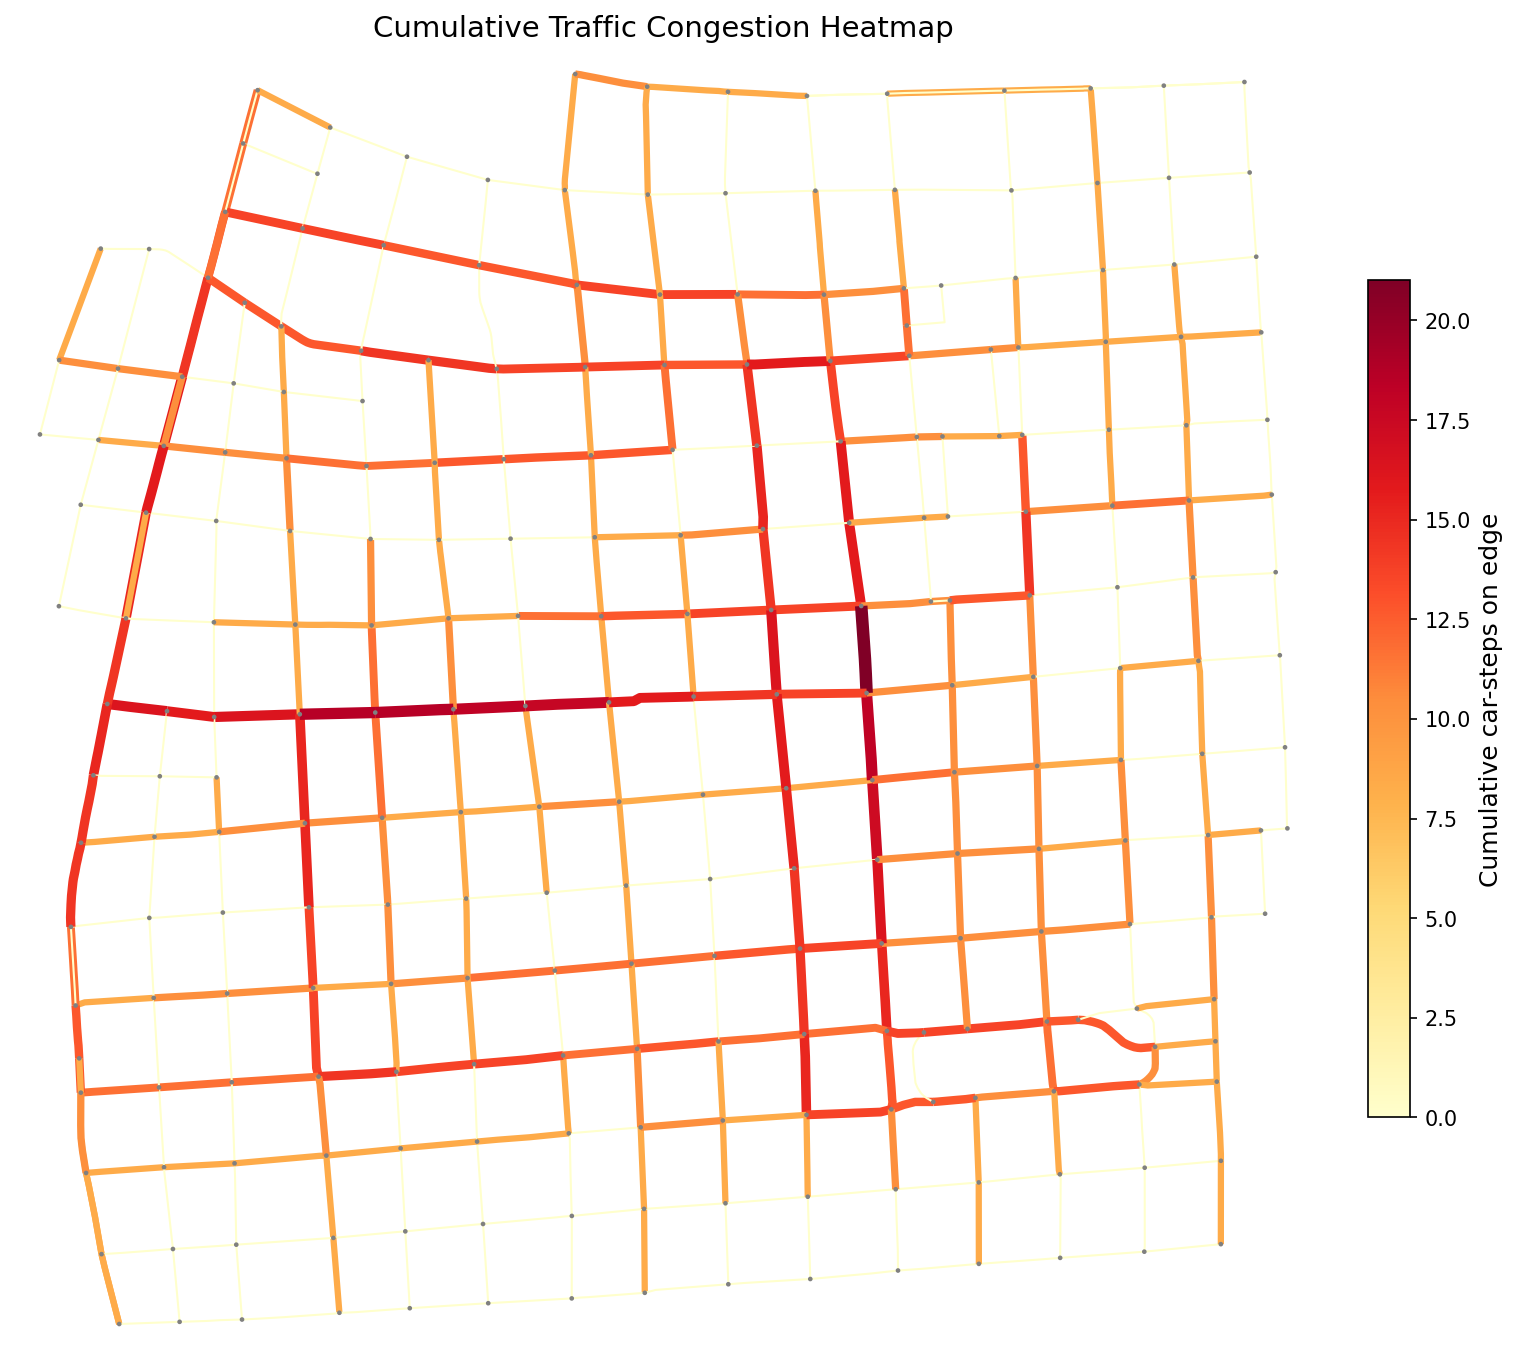
\includegraphics[width=0.85\textwidth]{cell_11_0.png}
    \caption{Cumulative congestion heatmap of the Avenida Corrientes network after running 100 cars for 10 steps using the original binary threshold model. Edge color (yellow to dark red) and width scale with total car-steps accumulated over the simulation. Although the visualization colors edges, the underlying congestion check is node-based: cars exist only at nodes, and the count reflects node-to-node jumps, not edge-level density. This measures traffic \textit{volume}, not actual congestion.}
    \label{fig:orig_heatmap}
\end{figure}

\begin{figure}[H]
    \centering
    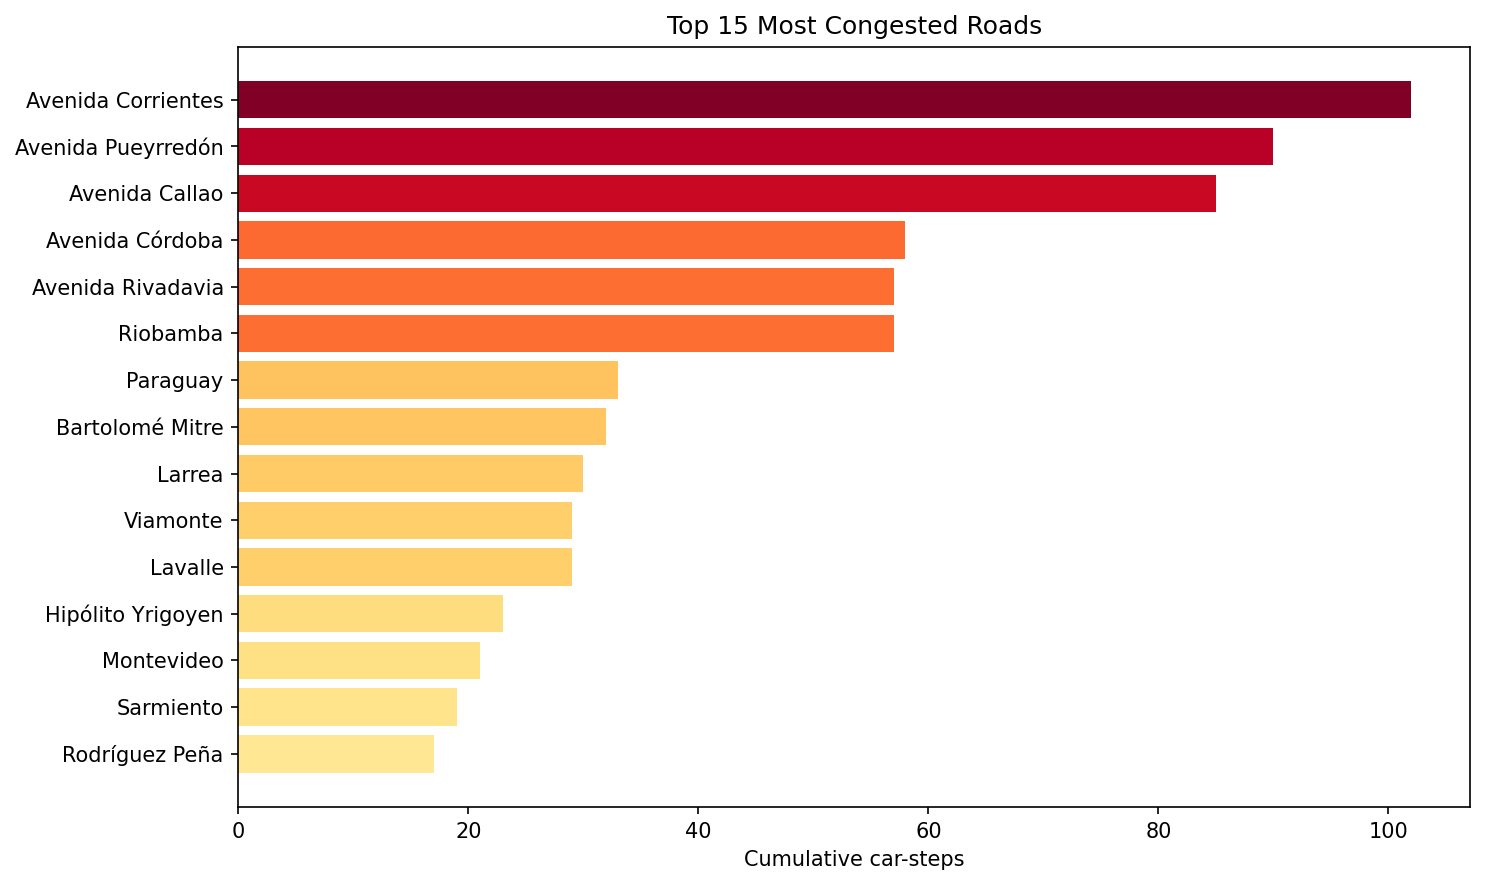
\includegraphics[width=0.8\textwidth]{cell_12_0.png}
    \caption{Top 15 streets in the Corrientes network ranked by cumulative car-steps from the original model. Streets composed of multiple edge segments are aggregated by name so the full road appears as a single bar. Because the model only tracks cars at nodes, these counts reflect route popularity (how many cars passed through), not congestion. A road with steady flow and a road approaching gridlock can produce similar counts.}
    \label{fig:orig_barchart}
\end{figure}

\begin{figure}[H]
    \centering
    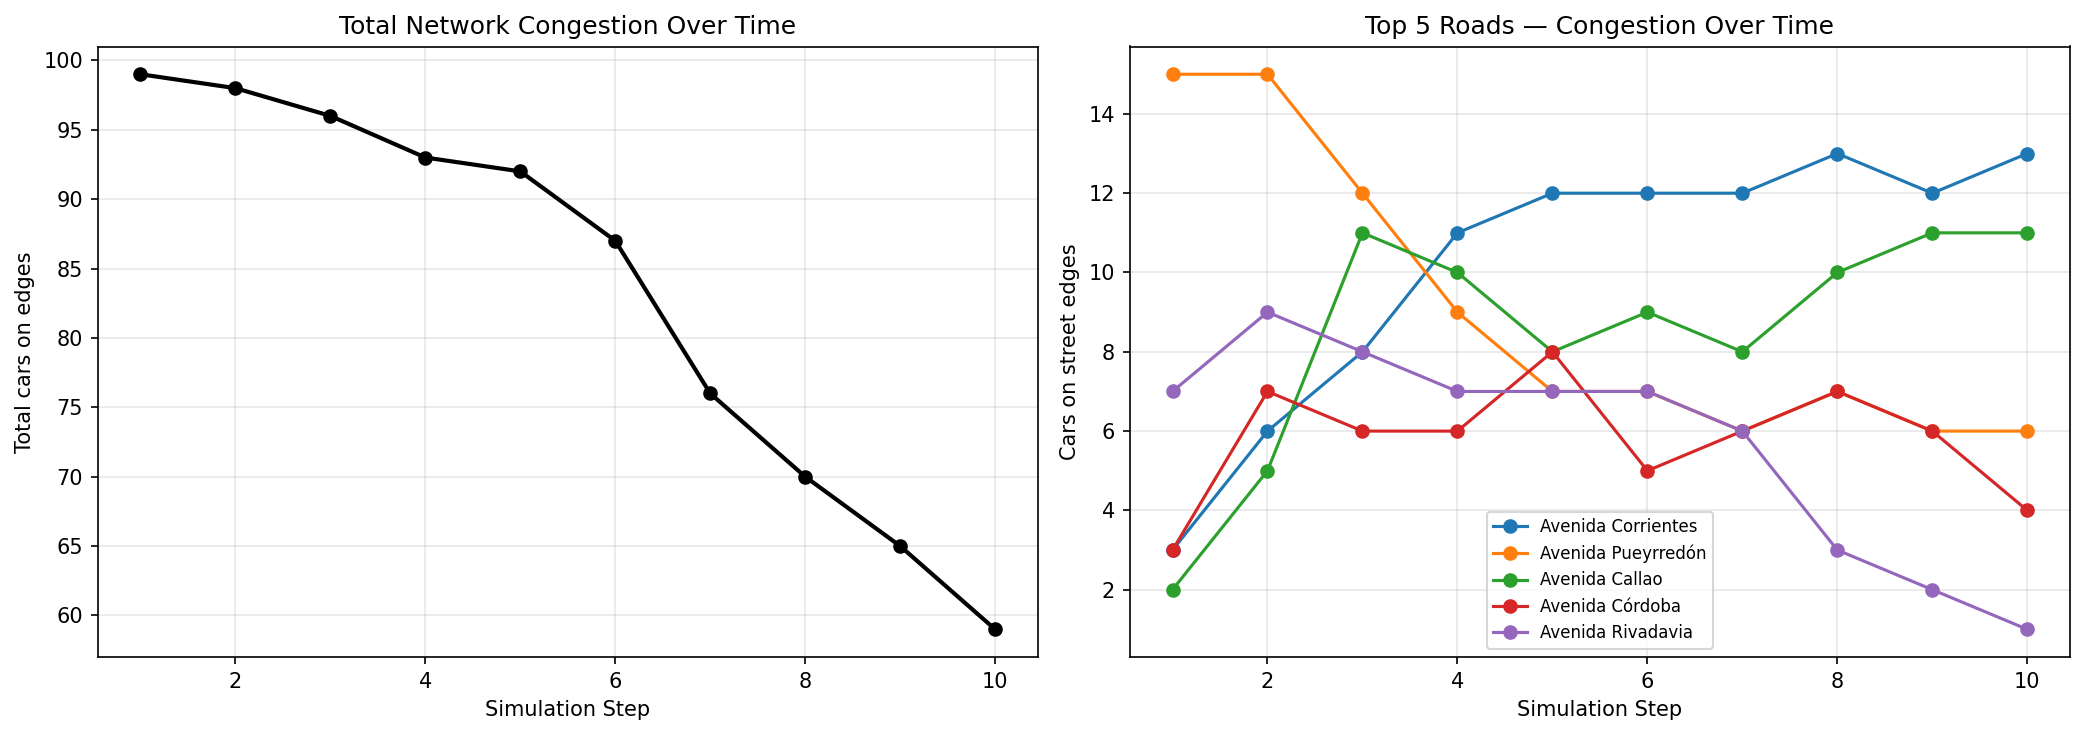
\includegraphics[width=\textwidth]{cell_13_0.png}
    \caption{Congestion dynamics over 10 simulation steps. Left panel: total cars still in transit across the network at each step, where the falling line shows cars reaching their destinations. Right panel: per-step car counts on the top 5 most-used streets. Because the model only checks congestion at nodes, these counts reflect how many cars used each street per step, not how congested the road actually was.}
    \label{fig:orig_timeseries}
\end{figure}

\subsection{What These Visualizations Actually Show}

These visualizations show traffic \textit{volume} (where cars went), not \textit{congestion} (where cars slowed down). ``Cumulative car-steps'' counts successful node-to-node traversals; it does not measure delay, slowdown, or density. A road with 1 car every step and a road with 5 cars every step look different in volume, but both are flowing freely under the threshold. The next section explains the structural reasons for this limitation.


% ============================================================================
\section{Why the Original Model Is Insufficient}
% ============================================================================

\subsection{Structural Problems}

\begin{itemize}
    \item \textbf{Binary congestion.} Below the threshold, cars move at full speed. Above it, they stop completely. Real traffic slows down gradually as density increases.
    \item \textbf{Arbitrary threshold.} The threshold of 5 cars has no relationship to road properties. A narrow residential street and a 6-lane avenida have the same capacity.
    \item \textbf{No position tracking.} Cars exist only at nodes, not along edges. A 50m alley and a 500m avenue process cars at the same rate (one node per step). Edge length is ignored entirely, and density (cars/meter) cannot be computed.
\end{itemize}

\subsection{Why This Produces Misleading Results}

Because congestion is binary, the visualizations can only show where cars \textit{went}, not where they \textit{slowed down}. Edges that appear ``congested'' in the heatmap may simply be popular routes with no actual delay. The model cannot distinguish between a busy road flowing smoothly and a gridlocked road, since both are invisible to the threshold check as long as they stay under 6 cars.


% ============================================================================
\section{Improved Model: Greenshields Density-Speed}
% ============================================================================

\subsection{The Greenshields Model}

We needed a model that incorporates road-level density (cars per meter) and converts it into a continuous speed. The Greenshields speed-density relationship \citep{greenshields1935} does exactly this with a single linear equation whose two parameters, $v_{\text{free}}$ (speed limit) and $\rho_{\text{jam}}$ (jam density from lane count), are both already available in the OpenStreetMap data. No calibration is required, and because our analysis focuses on \textit{relative} congestion patterns rather than exact travel times, the linear approximation is sufficient. The relationship is:
\begin{equation}
    v = v_{\text{free}} \times \max\!\left(1 - \frac{\rho}{\rho_{\text{jam}}},\; 0.05\right)
    \label{eq:greenshields}
\end{equation}
where $v_{\text{free}}$ is the free-flow speed (the posted speed limit from OSM data, i.e.\ the speed a car travels when alone on the road), $\rho$ is the current density (cars/meter on the edge), and $\rho_{\text{jam}}$ is the jam density (the maximum number of cars per meter that can physically fit on the road, determined by the number of lanes, so more lanes means more cars can pack in before the road is fully jammed). In our implementation, $\rho_{\text{jam}} = 0.04 \times \text{lanes}$~cars/meter; the standard traffic engineering value is ${\sim}0.15$~cars/m/lane (${\sim}$one car every 7~m), but we scale it down so that congestion effects are visible with the simulation's relatively small car counts. Speed decreases continuously as density increases: at zero density, cars travel at free-flow speed; at jam density, they slow to 5\% of free-flow speed (the floor prevents cars from fully stopping, which would deadlock the simulation).

\subsection{Implementation}

The improved model is implemented via two subclasses that inherit from the original classes, overriding only the movement logic:

\begin{itemize}
    \item \textbf{ImprovedCar(Car)}: adds \texttt{position} (meters along the current edge), \texttt{current\_edge}, and \texttt{speed} attributes.
    \item \textbf{ImprovedTrafficSimulation(TrafficSimulation)}: overrides \texttt{\_move\_cars()} to implement Greenshields:
    \begin{enumerate}
        \item Cars are spawned at random positions along random edges (not just at nodes).
        \item Each step: count cars per edge, compute density $\rho = \text{cars} / \text{edge\_length}$.
        \item Derive speed from Equation~\ref{eq:greenshields}.
        \item Advance each car's position by its speed. When position exceeds the edge length, the car transitions to the next edge.
        \item Jam density $\rho_{\text{jam}}$ varies by lane count from OSM data.
    \end{enumerate}
\end{itemize}

Each time step represents approximately 6 seconds; free-flow speed at 30~km/h is approximately 50~m/step. All visualization methods are inherited from the parent class.

\subsection{What This Fixes}

This model directly addresses each structural problem identified in Section~4:

\begin{itemize}
    \item \textbf{Binary congestion $\to$ continuous.} Instead of a hard threshold where cars either move at full speed or stop entirely, the Greenshields equation produces a smooth speed curve. A road with 3 cars behaves differently from a road with 10 cars, which behaves differently from a road with 50 cars.
    \item \textbf{Arbitrary threshold $\to$ physical parameters.} The original model's threshold of 5 had no connection to road properties. Greenshields replaces it with $\rho_{\text{jam}}$, which varies by lane count: a 3-lane avenue can hold three times as many cars per meter as a single-lane street before reaching jam density.
    \item \textbf{No position tracking $\to$ edge-level density.} Cars now have positions along edges (in meters), so density can be computed as cars per meter. A 50~m alley with 2 cars is much more congested than a 500~m avenue with 2 cars, and the model captures this difference.
\end{itemize}

\subsection{Connection to Cellular Automata}

The improved simulation can be understood as a cellular automaton (CA) operating on a network graph. Each edge is a ``cell'' whose state is its current density (cars/meter). The update rule is the Greenshields equation (Equation~\ref{eq:greenshields}): at each discrete time step, each edge's density determines the speed of its cars, which in turn determines how many cars leave the edge and enter adjacent edges in the next step. The state of each cell at time $t+1$ depends on its own state and the states of its neighbors at time $t$, which is the defining property of a cellular automaton.

This contrasts with the Nagel-Schreckenberg (NaSch) model \citep{nagel1992}, the canonical traffic CA. NaSch operates on a one-dimensional lattice where each cell is a road position and the state is ``car or empty.'' Each car follows four micro-rules per step: accelerate (up to a max speed), brake (if the car ahead is too close), randomly decelerate (modeling human unpredictability), and move forward. Our model operates on a network graph where cells are edges and the state is a continuous density value, updated by a single macro-rule (Greenshields).

Both are cellular automata, but at different scales. NaSch is \textit{microscopic}: it tracks individual car decisions (accelerate, brake, hesitate). Our model is \textit{macroscopic}: it tracks aggregate density and derives speed from it. The microscopic approach captures phenomena like phantom traffic jams (spontaneous stop-and-go waves), while the macroscopic approach captures how network topology distributes and concentrates congestion. Section~\ref{sec:gridlock} uses this framing to compare how different graph topologies handle increasing traffic.


% ============================================================================
\section{Limitations and Assumptions}
% ============================================================================

The improved model addresses the structural problems of the original, but it introduces its own simplifications. Each simplification is a trade-off, but none of them affect the relative congestion patterns that our analysis depends on.

\paragraph{Linear speed-density relationship.}
The Greenshields model assumes that speed decreases \textit{linearly} with density. In reality, the speed-density relationship is nonlinear; alternative models such as Greenberg (logarithmic) and Underwood (exponential) better capture the sharp speed drop near jam density. We chose Greenshields because it has only two parameters ($v_{\text{free}}$ and $\rho_{\text{jam}}$), is analytically transparent, and produces qualitatively correct behavior: free flow at low density, gradual slowdown, and gridlock at jam density. Since our analysis focuses on \textit{relative} congestion patterns (which edges congest more than others) rather than precise speed values, the linear approximation is sufficient.

\paragraph{Static routing.}
Cars compute their shortest path once at spawn and follow it to their destination, regardless of congestion encountered along the way. Real drivers adapt: they check navigation apps, take side streets, or avoid visibly jammed roads. This means our simulation overestimates congestion on shortest-path bottlenecks and underestimates load on alternative routes. The effect is especially relevant for the grid topology analysis (Section~\ref{sec:gridlock}), where the grid's many parallel paths would become more useful under dynamic rerouting.

\paragraph{No intersection delay.}
Cars transition instantly between edges at nodes. Real intersections impose delays: traffic lights, stop signs, turning conflicts, and pedestrian crossings all add time that depends on intersection geometry and signal timing. This simplification means our simulation underestimates total travel time and cannot capture intersection-specific bottlenecks. However, since we compare congestion \textit{across edges} rather than predicting absolute travel times, the omission is acceptable for our purposes.

\paragraph{Uniform car behavior.}
All cars follow the same Greenshields rule with identical parameters. There is no variation in driver aggression, vehicle size, reaction time, or willingness to take longer routes. This is a consequence of the macroscopic modeling choice: individual car heterogeneity is averaged out in favor of aggregate density dynamics. A microscopic model like Nagel-Schreckenberg would capture these differences but at much greater computational cost and complexity.


% ============================================================================
\section{New Visualizations}
% ============================================================================

\subsection{Car Animation}

An animated visualization shows cars (blue dots) moving through the network in real time. Cars visibly slow down on congested edges and flow freely on empty ones, directly demonstrating the Greenshields model. Figure~\ref{fig:car_anim} shows a representative frame.

\begin{figure}[H]
    \centering
    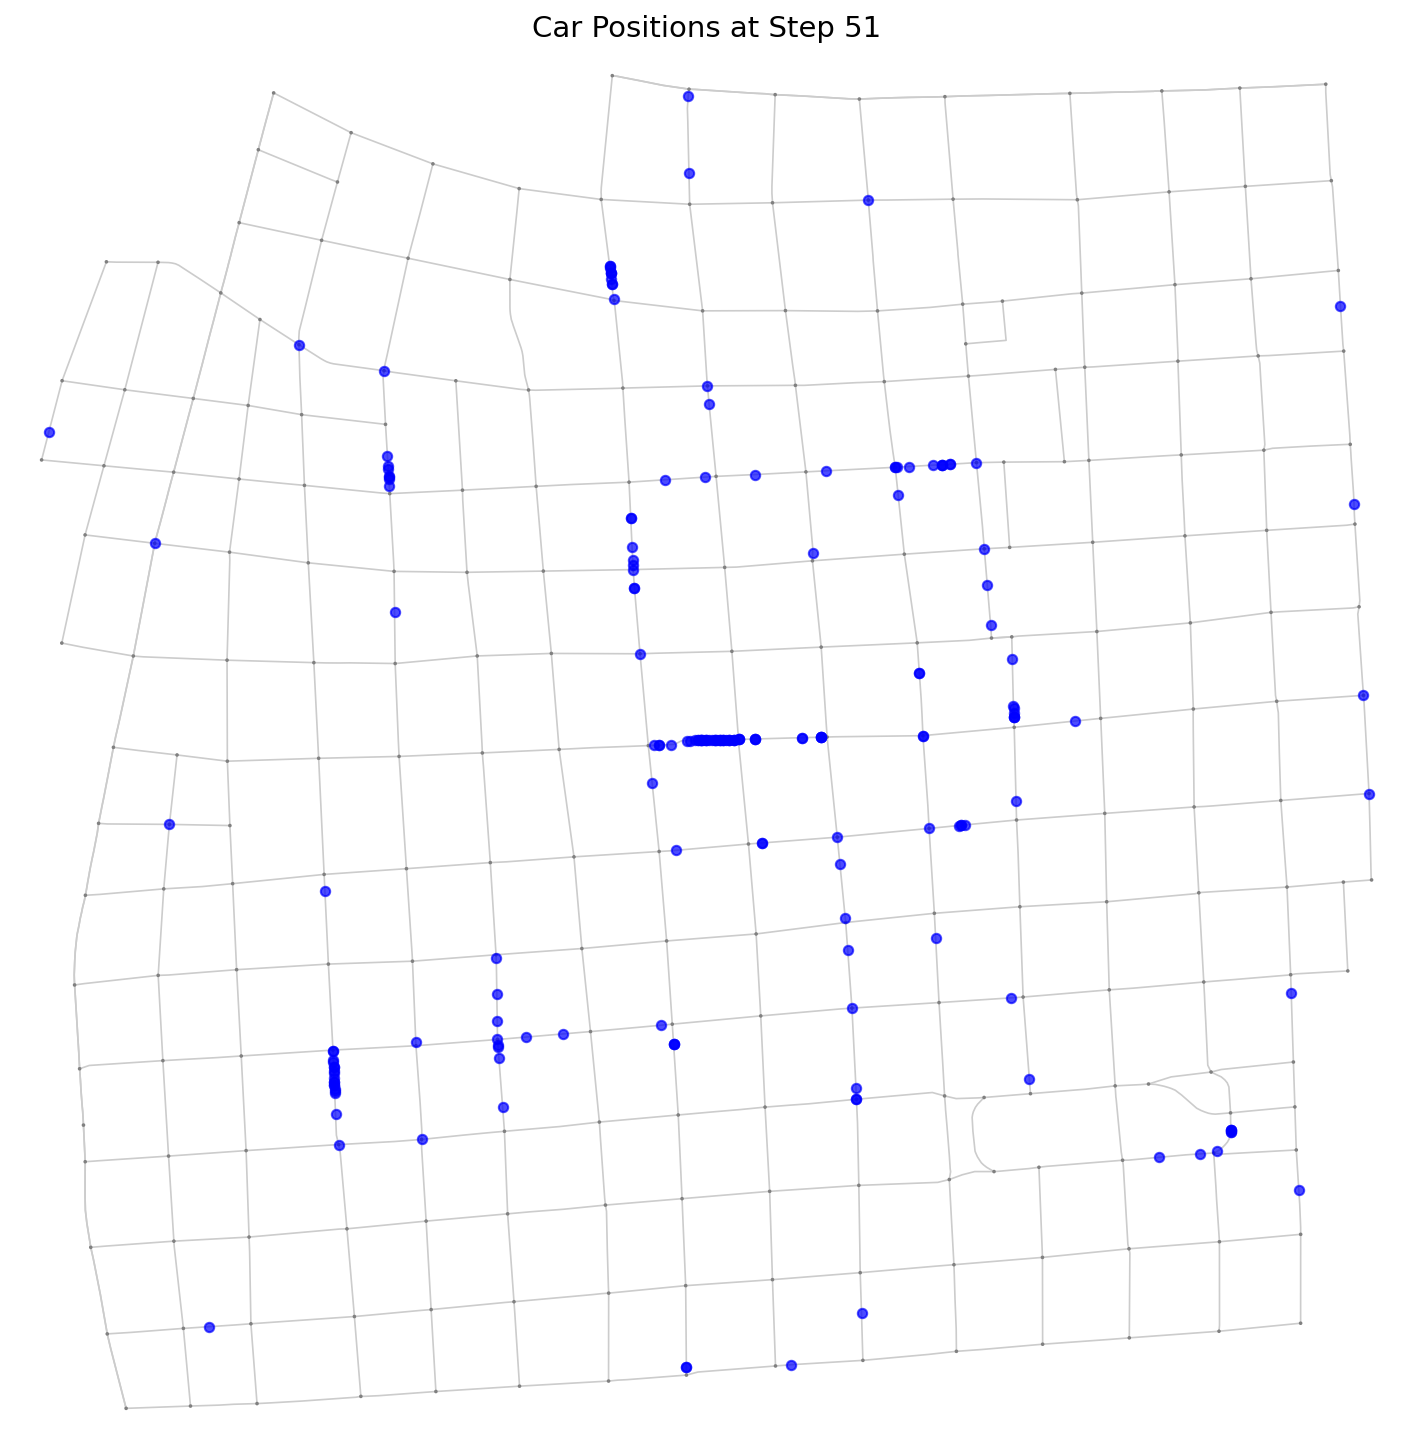
\includegraphics[width=0.85\textwidth]{cell_21_frame.png}
    \caption{Representative frame from the car animation at step 51 of 100, showing 500 cars (blue dots) distributed across the Corrientes road network. Car positions are interpolated along edges based on their Greenshields-derived speeds. Clusters of dots on certain edges indicate congestion, where cars are slowing down due to high local density. The full interactive animation with play/pause controls is available in the notebook.}
    \label{fig:car_anim}
\end{figure}

\subsection{Density Heatmap Animation}

Edge colors show local density (cars/meter) evolving over time. Congestion builds at bottleneck edges and dissipates as cars clear. Figure~\ref{fig:density_anim} shows a representative frame.

\begin{figure}[H]
    \centering
    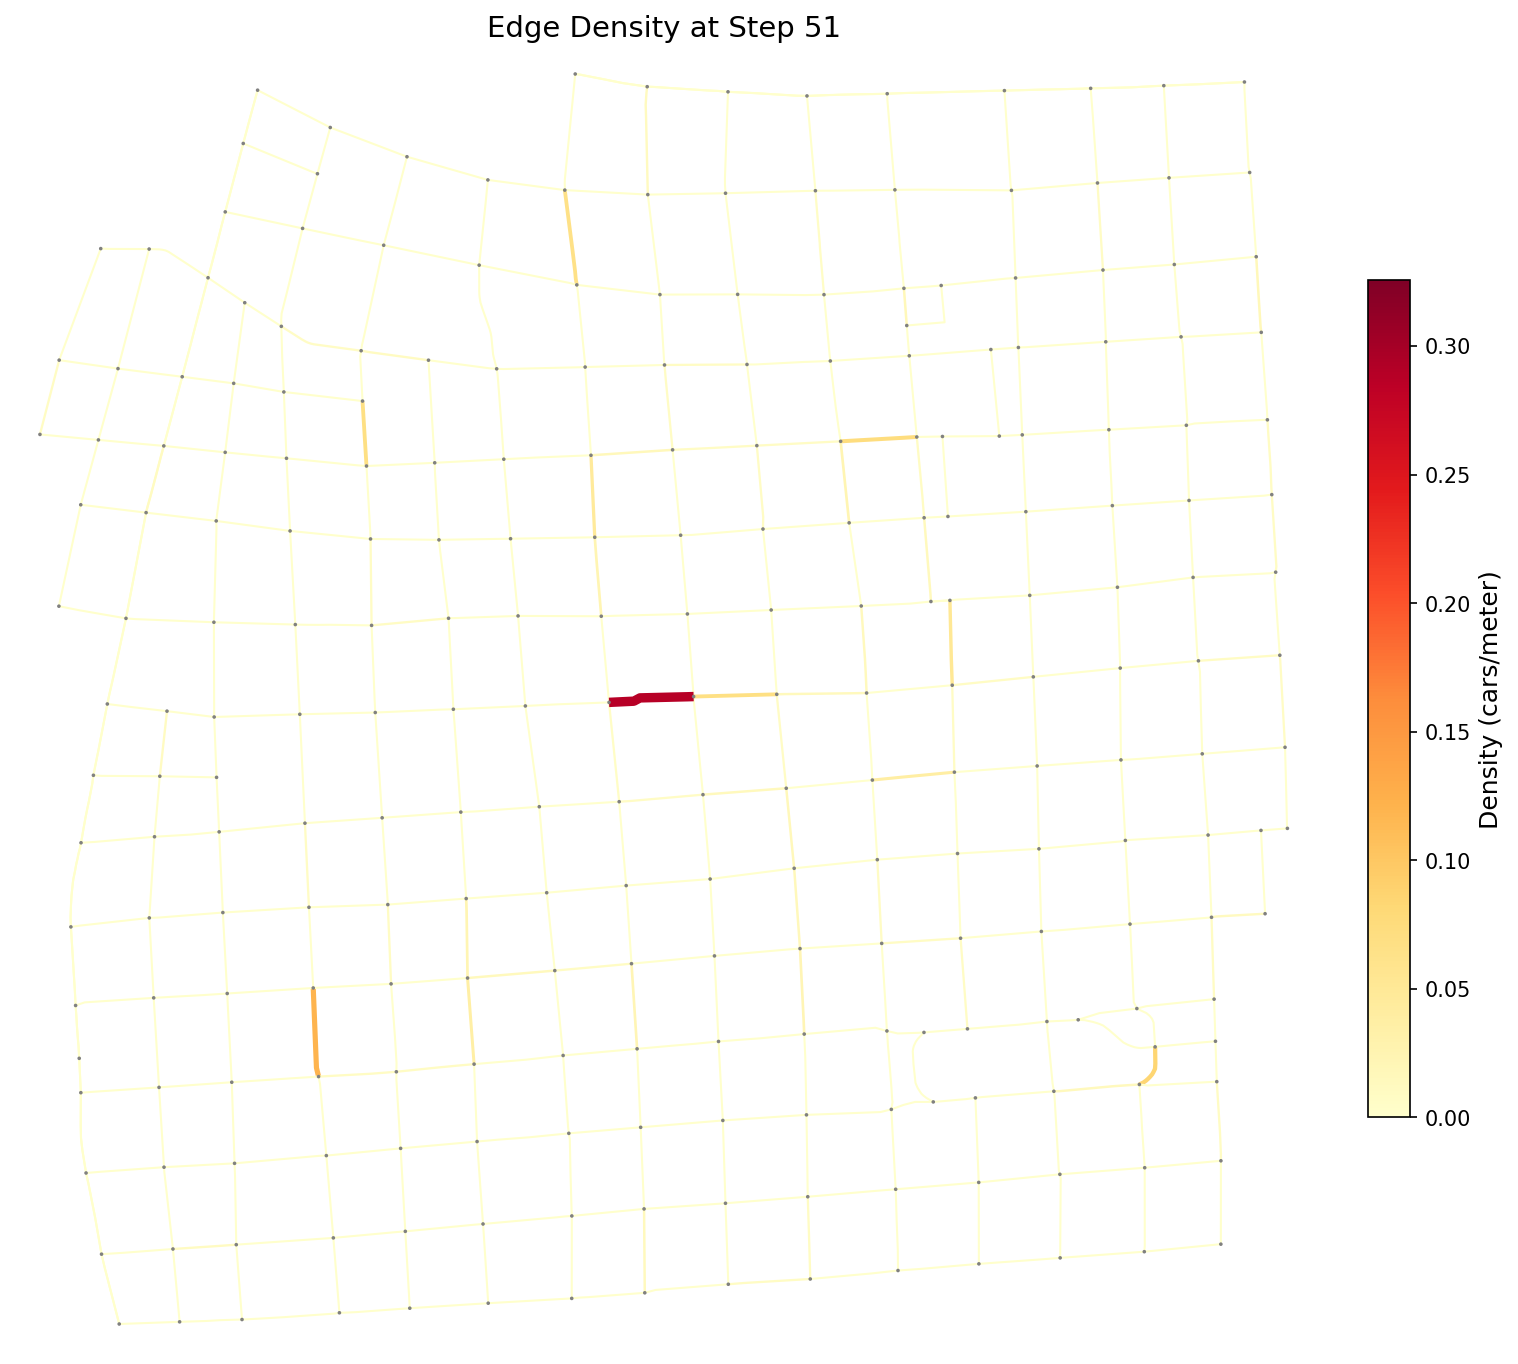
\includegraphics[width=0.85\textwidth]{cell_23_frame.png}
    \caption{Representative frame from the density heatmap animation at step 51 of 100. Each edge is colored by its instantaneous density (cars/meter): yellow indicates low or zero density, dark red indicates high density approaching jam conditions. Edge widths also scale with density. The colorbar provides the quantitative mapping. The full animation shows congestion building at bottlenecks and dissipating as cars clear.}
    \label{fig:density_anim}
\end{figure}

\subsection{Average Density Heatmap}

A static summary of the average density per edge across all simulation steps (Figure~\ref{fig:avg_density}). This is the congestion measure used in the subsequent multi-run analysis.

\begin{figure}[H]
    \centering
    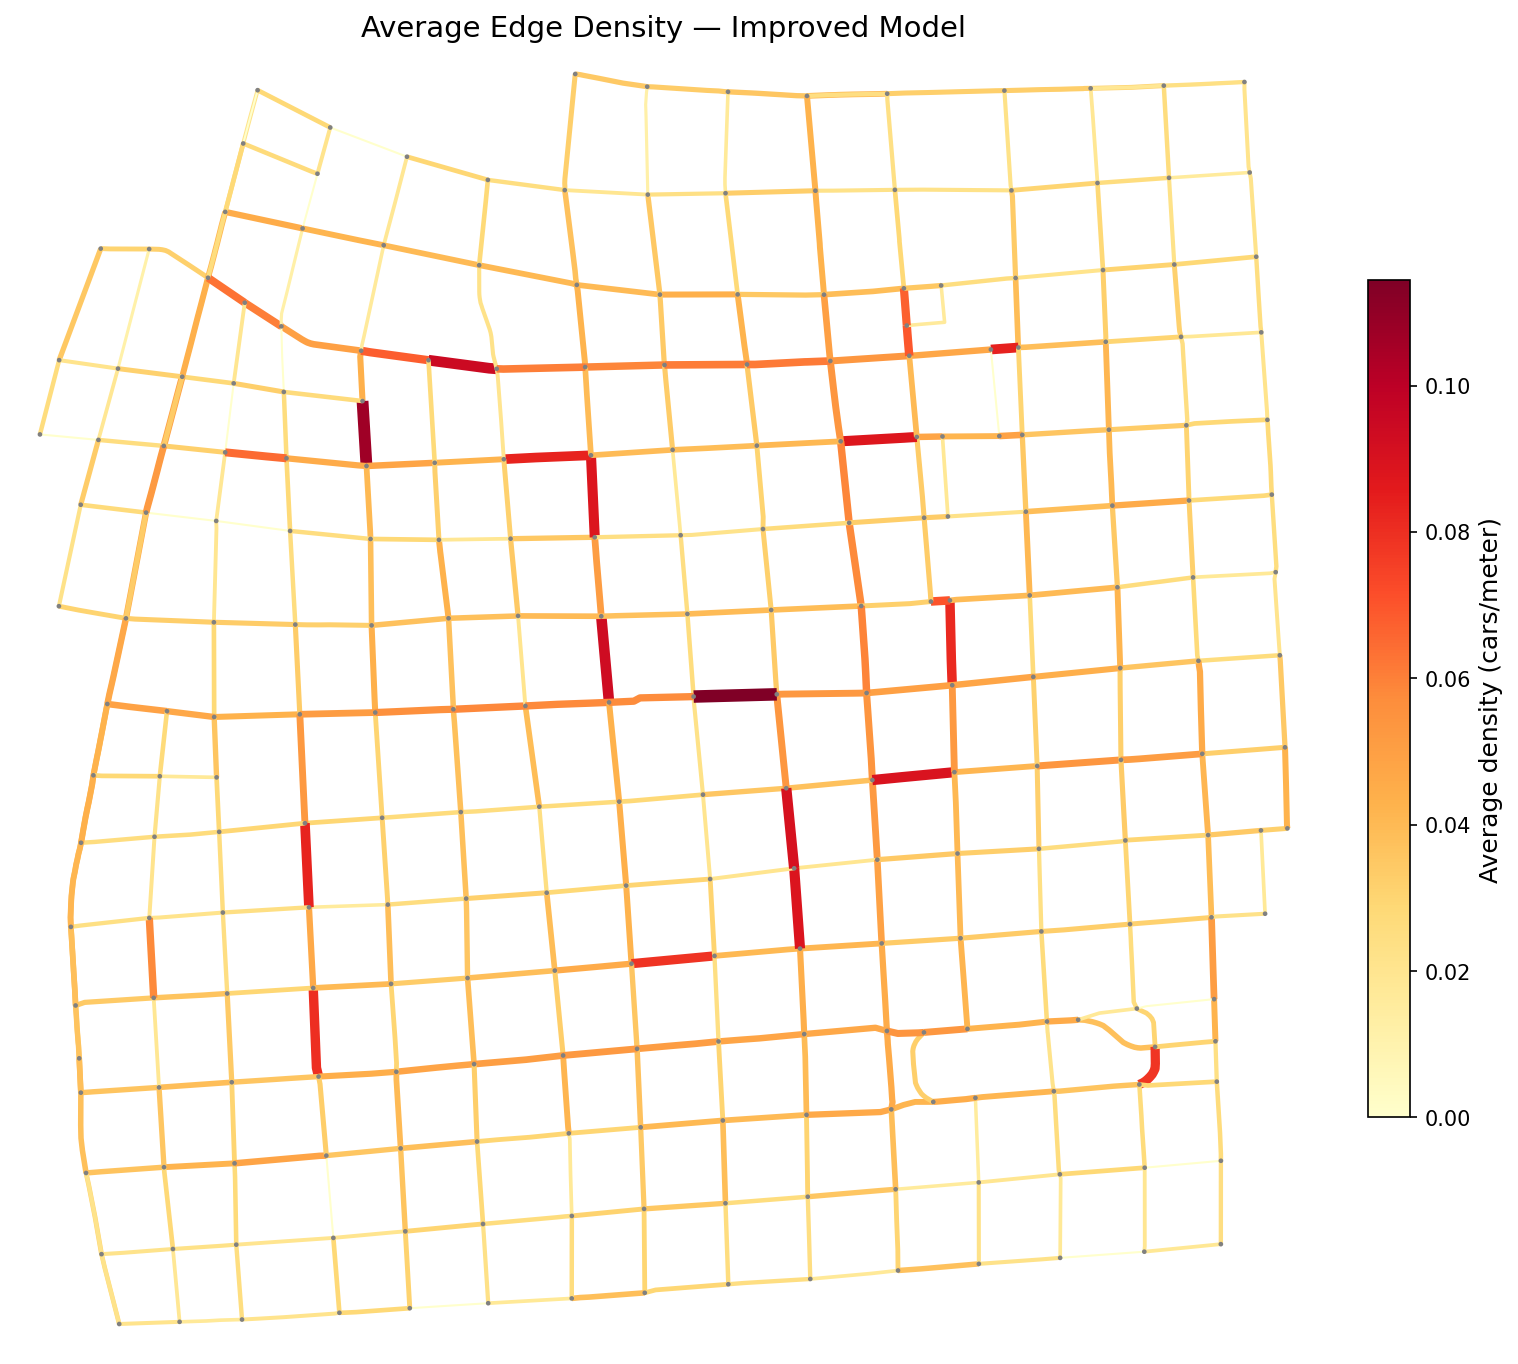
\includegraphics[width=0.85\textwidth]{cell_23_0.png}
    \caption{Average edge density (cars/meter) over a single simulation run with 500 cars and 100 steps using the Greenshields model. Unlike the original model's cumulative car-steps, density accounts for road length. A short edge with few cars can show higher density than a long edge with many cars. The colorbar maps edge color to average density. This is the congestion measure used in the subsequent multi-run analysis.}
    \label{fig:avg_density}
\end{figure}

\subsection{Comparison: Original vs Improved}

The original visualizations (Section~3) show where cars \textit{went}. These new visualizations show where cars actually slowed down.


% ============================================================================
\section{Empirical Congestion Analysis}
% ============================================================================

\subsection{Methodology}

A single simulation run is noisy because random car placements mean different roads get congested each time. To find roads that are \textit{structurally} prone to congestion, we run 50 independent simulations using the improved Greenshields model (500 cars, 100 steps each) and average the density per edge across all runs. Roads that consistently show high density are true bottlenecks, not artifacts of randomness.

\subsection{Results}

\begin{figure}[H]
    \centering
    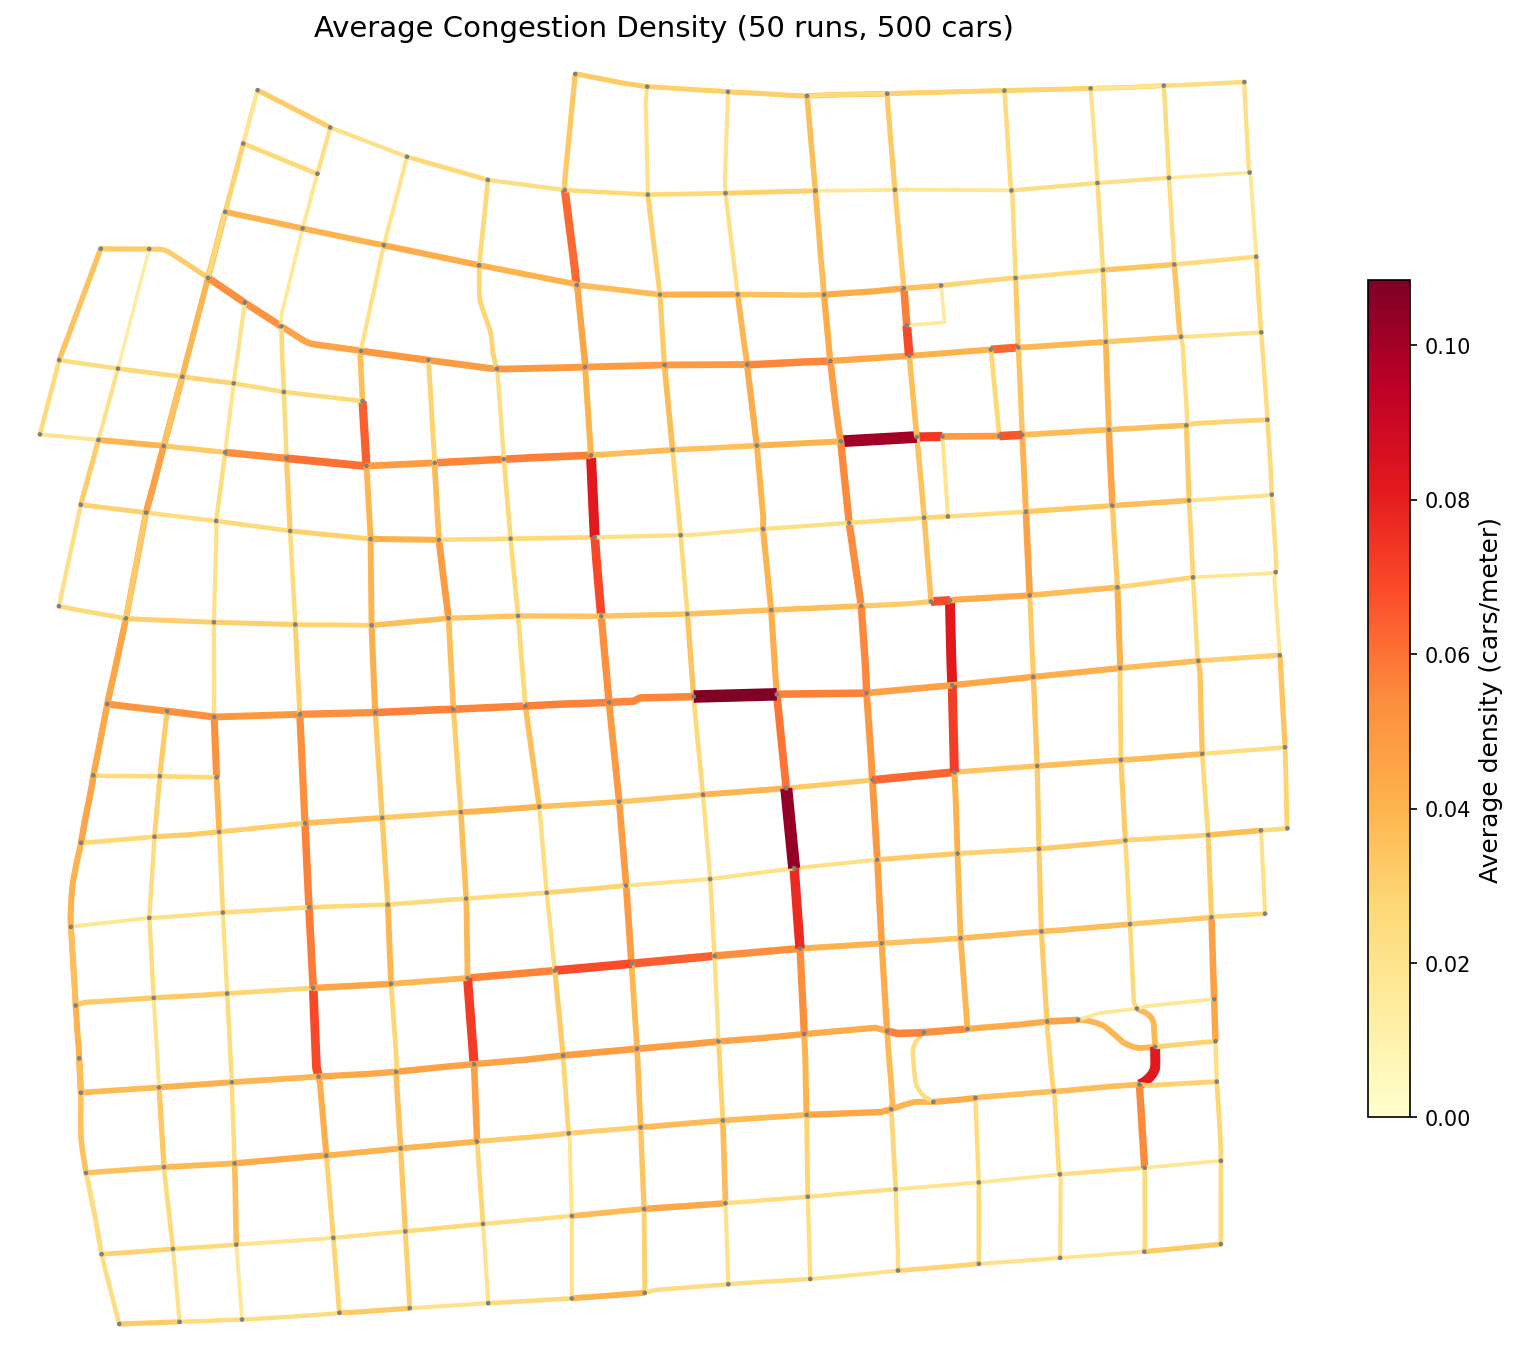
\includegraphics[width=0.85\textwidth]{cell_26_0.png}
    \caption{Average congestion density (cars/meter) across 50 independent simulation runs, each with 500 cars and 100 steps. Averaging removes noise from random car placements and reveals edges that are \textit{structurally} prone to congestion due to their position in the network. Darker red and thicker edges indicate consistently higher density. The pattern is stable across runs, confirming these are true bottlenecks rather than random artifacts.}
    \label{fig:avg_density_50}
\end{figure}


% ============================================================================
\section{Network Metrics as Congestion Predictors}
% ============================================================================

\subsection{Why Edge Betweenness Centrality}

Most standard network metrics (degree centrality, closeness, clustering coefficient, etc.) are defined at the \textit{node} level. However, congestion happens on \textit{edges} (road segments between intersections), and mapping node metrics to edges by averaging endpoints is not principled.

\textbf{Edge betweenness centrality} is one of the few metrics defined directly on edges. It measures the fraction of all shortest paths in the network that traverse a given edge. Since our cars route via shortest paths, this is a direct structural prediction of traffic demand. Edges on many shortest paths should attract more cars and therefore experience higher density.

\subsection{Correlation Analysis}

We compute edge betweenness centrality (weighted by \texttt{travel\_time} to match how cars route) and correlate it against the empirical density from the multi-run analysis. We use the Spearman rank correlation \citep{spearman1904} rather than Pearson because the relationship between betweenness and density is not linear (as visible in the scatter plot). Spearman measures whether the rankings agree, which is what we care about: can betweenness predict \textit{which} edges congest? The result is $r = 0.88$ ($p < 10^{-160}$).

\begin{figure}[H]
    \centering
    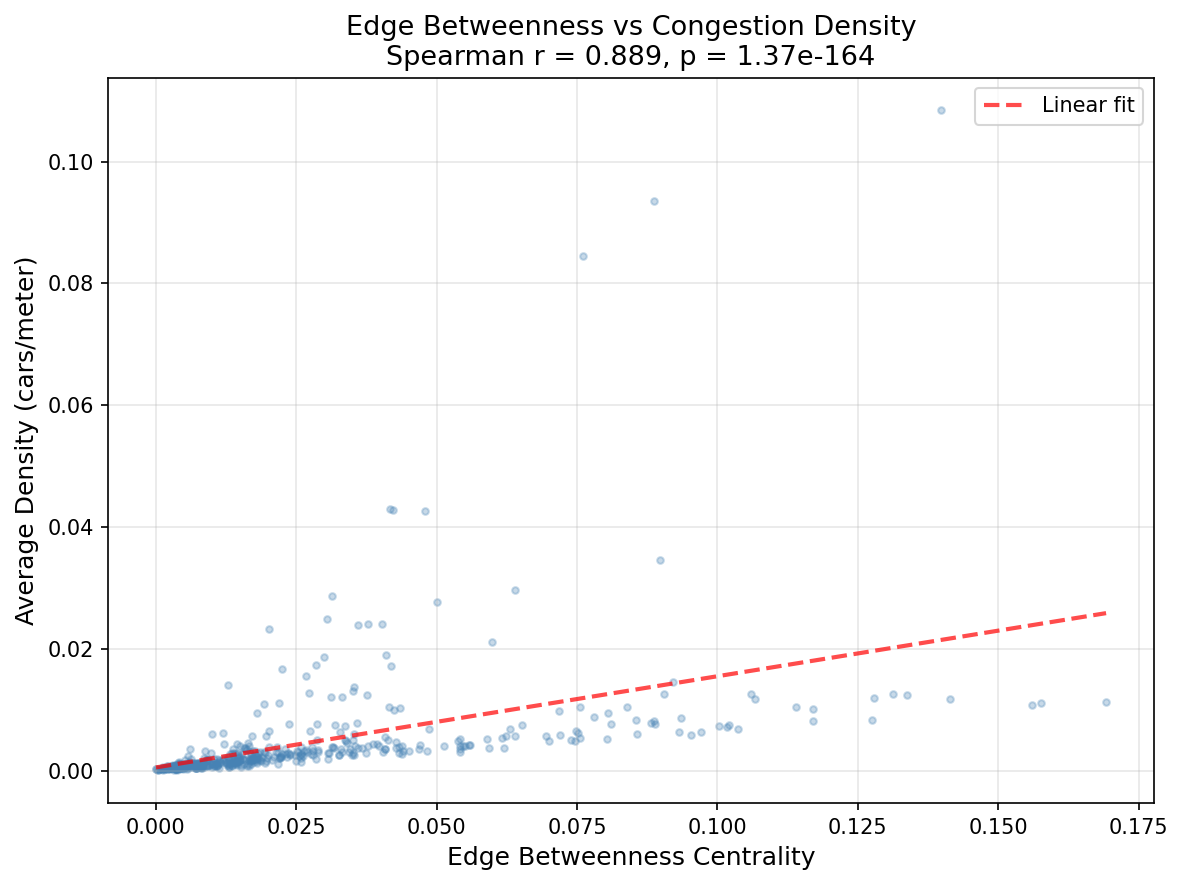
\includegraphics[width=0.75\textwidth]{cell_29_0.png}
    \caption{Scatter plot comparing edge betweenness centrality (x-axis) to empirical average density from 50 simulation runs (y-axis) on the Corrientes network. Each point represents one edge. The strong positive correlation (Spearman $r = 0.88$, $p < 10^{-160}$) confirms that edges lying on many shortest paths experience higher congestion density. The red dashed line shows the linear trend.}
    \label{fig:scatter_ebc}
\end{figure}

\subsection{Visual Comparison}

\begin{figure}[H]
    \centering
    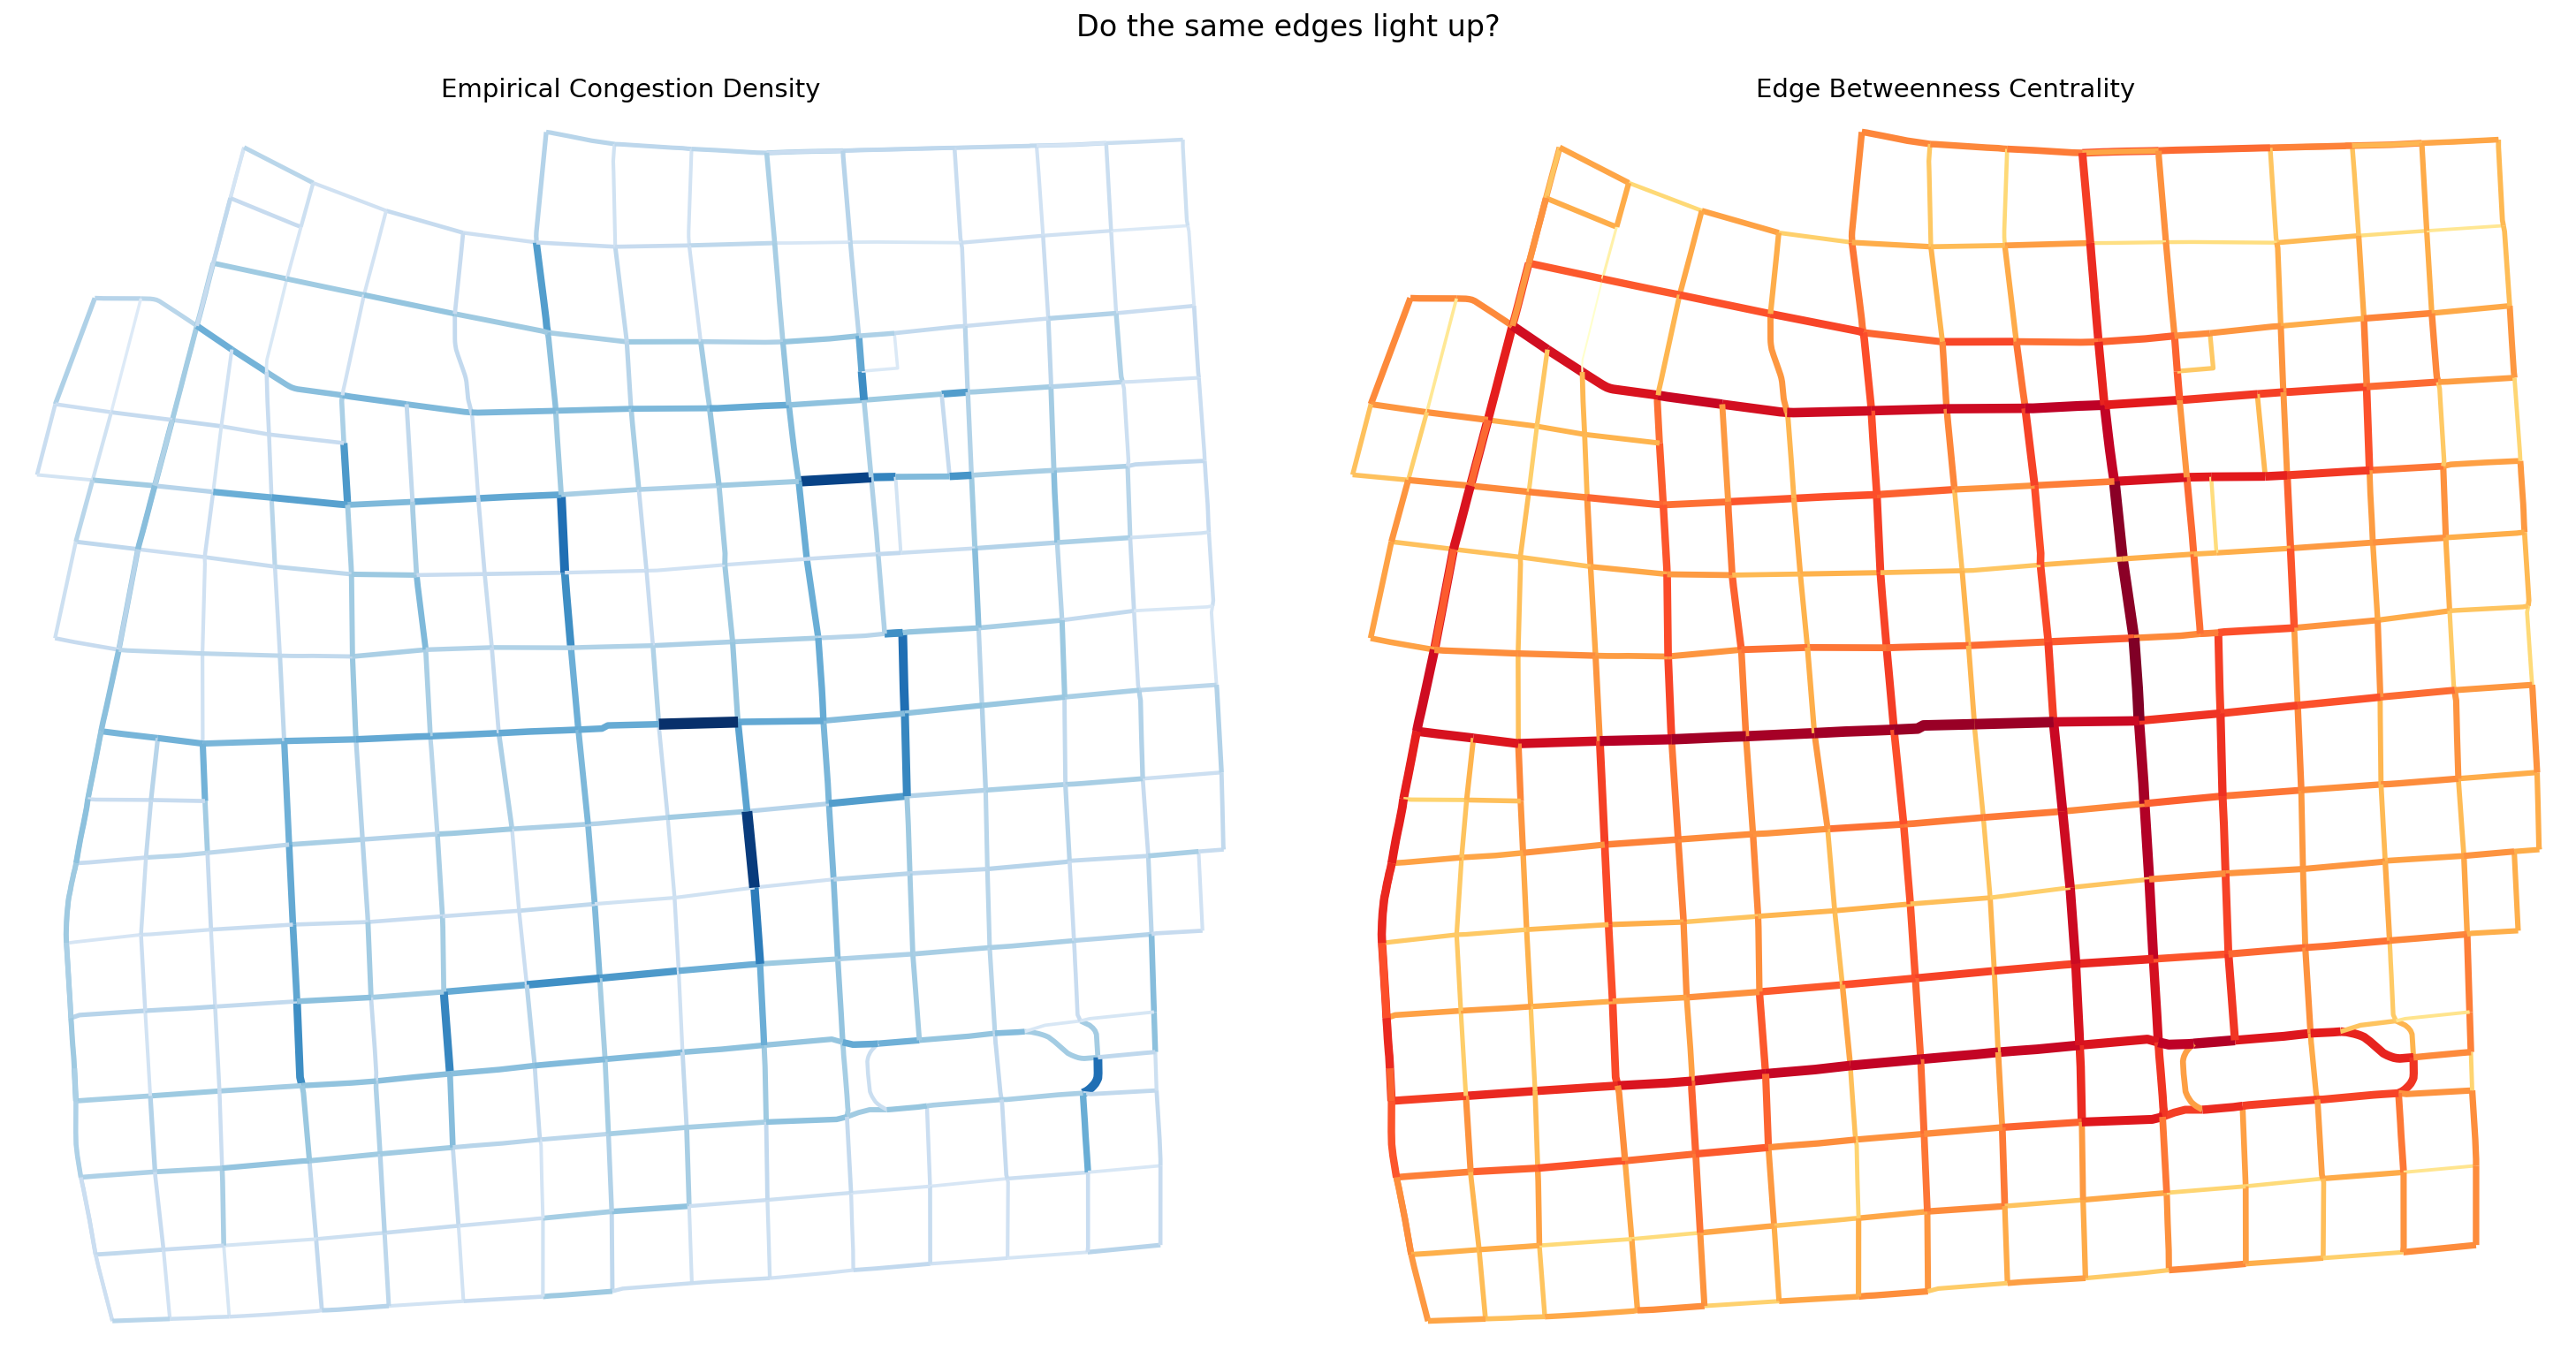
\includegraphics[width=\textwidth]{cell_30_0.png}
    \caption{Side-by-side spatial comparison on the Corrientes network. Left: empirical congestion density from 50 simulation runs. Right: edge betweenness centrality computed purely from network structure. The empirical map uses a Blues color scale and the betweenness map uses YlOrRd, so they can be compared without conflating the two measures. The highest-traffic edges in the empirical map generally correspond to the highest-betweenness edges, though the betweenness map highlights more edges overall since it captures potential rather than realized traffic.}
    \label{fig:sidebyside_corrientes}
\end{figure}

The two maps in Figure~\ref{fig:sidebyside_corrientes} show broad spatial agreement: the edges with the highest empirical density tend to also have high betweenness centrality. The match is not perfect (some high-betweenness edges show only moderate density, and a few high-density edges are not the top-ranked by betweenness), but the overall pattern is consistent with the Spearman $r = 0.88$.


% ============================================================================
\section{Validation on a Different Location}
% ============================================================================

\subsection{Validation Setup}

To test whether edge betweenness centrality generalizes as a congestion predictor, we repeat the analysis on a second road network: Plaza Italia / Palermo, Buenos Aires. This neighborhood has a different road topology from the Corrientes downtown area. The same methodology is used: 50 simulation runs, 500 cars, 100 steps.

\begin{figure}[H]
    \centering
    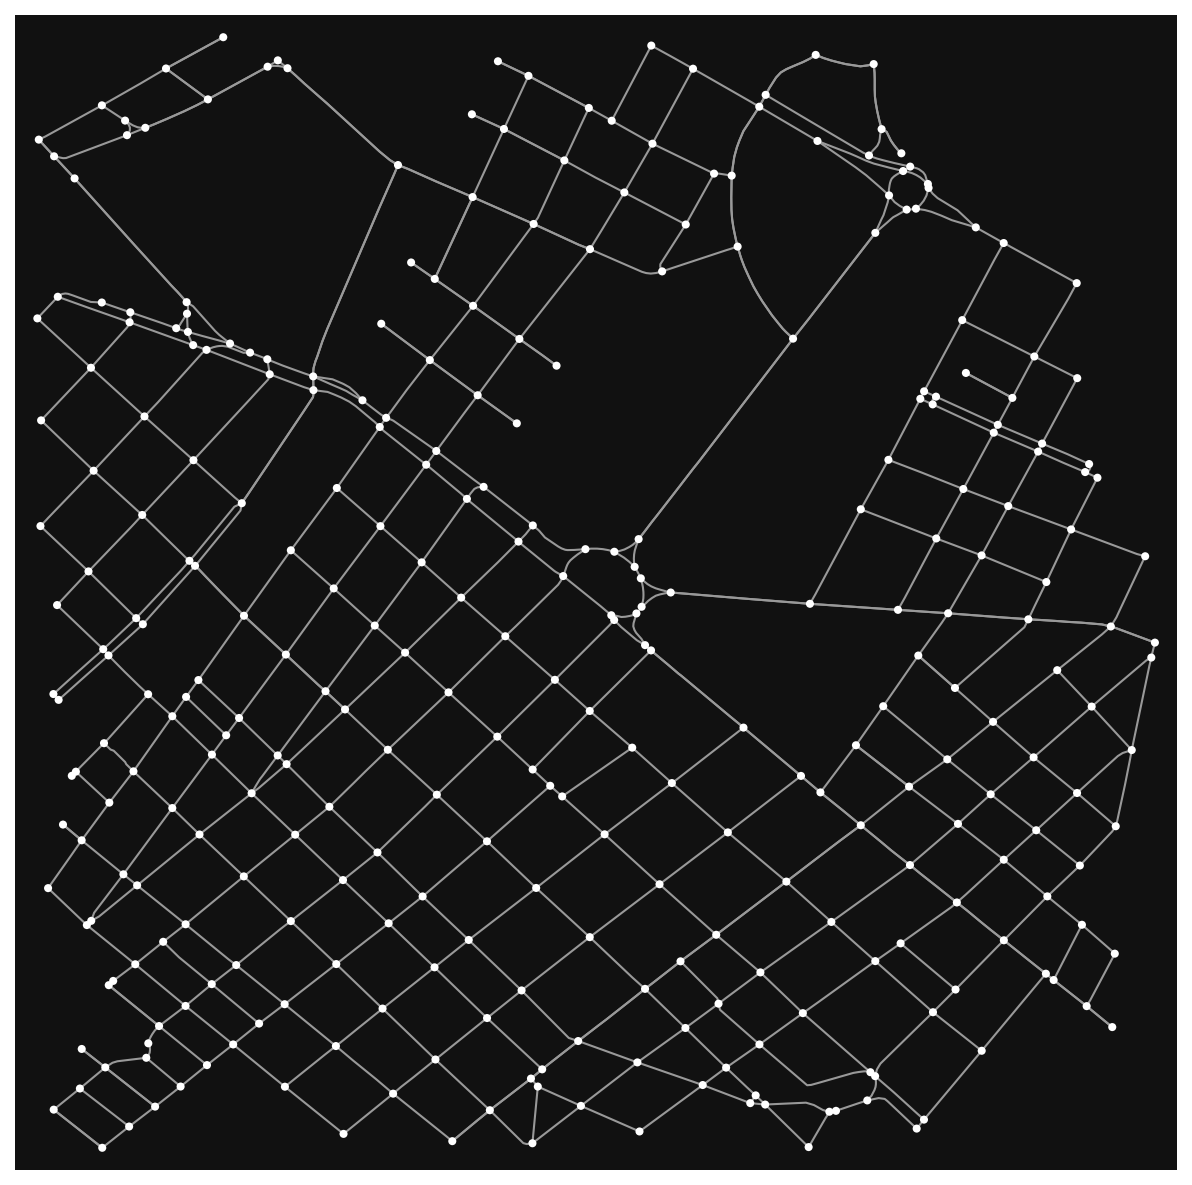
\includegraphics[width=0.7\textwidth]{cell_32_0.png}
    \caption{The Plaza Italia / Palermo road network used for validation, loaded from OpenStreetMap with a 1~km radius. This neighborhood has a different topology from the downtown Corrientes area, with wider boulevards, more parks, and a different grid structure. The network is reduced to its largest strongly connected component to ensure full reachability.}
    \label{fig:palermo_network}
\end{figure}

\subsection{Results}

\begin{figure}[H]
    \centering
    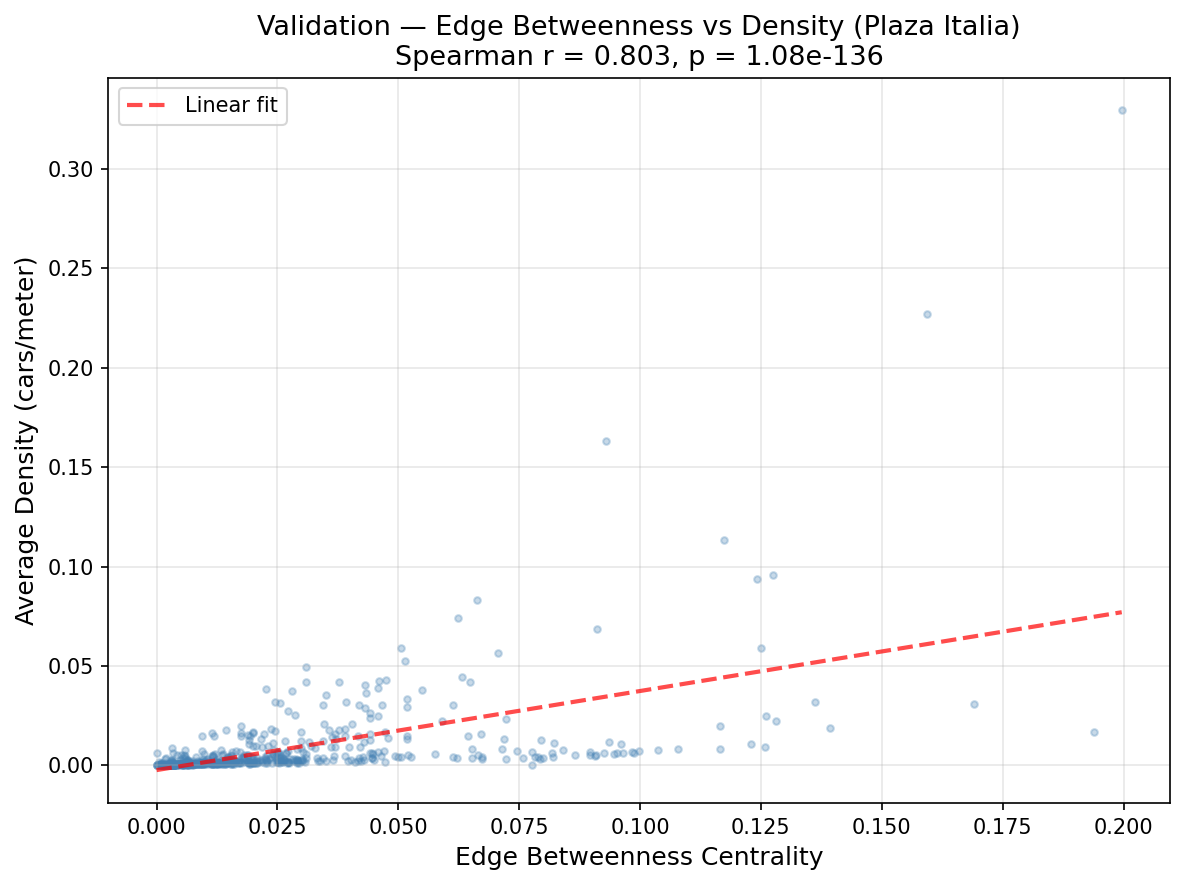
\includegraphics[width=0.75\textwidth]{cell_35_0.png}
    \caption{Scatter plot of edge betweenness centrality vs.\ empirical density on the Plaza Italia validation network ($r = 0.81$, $p < 10^{-139}$). The positive correlation persists on this different topology, though slightly weaker than the Corrientes network ($r = 0.88$). This confirms that edge betweenness generalizes as a congestion predictor across different road network structures.}
    \label{fig:scatter_palermo}
\end{figure}

\begin{figure}[H]
    \centering
    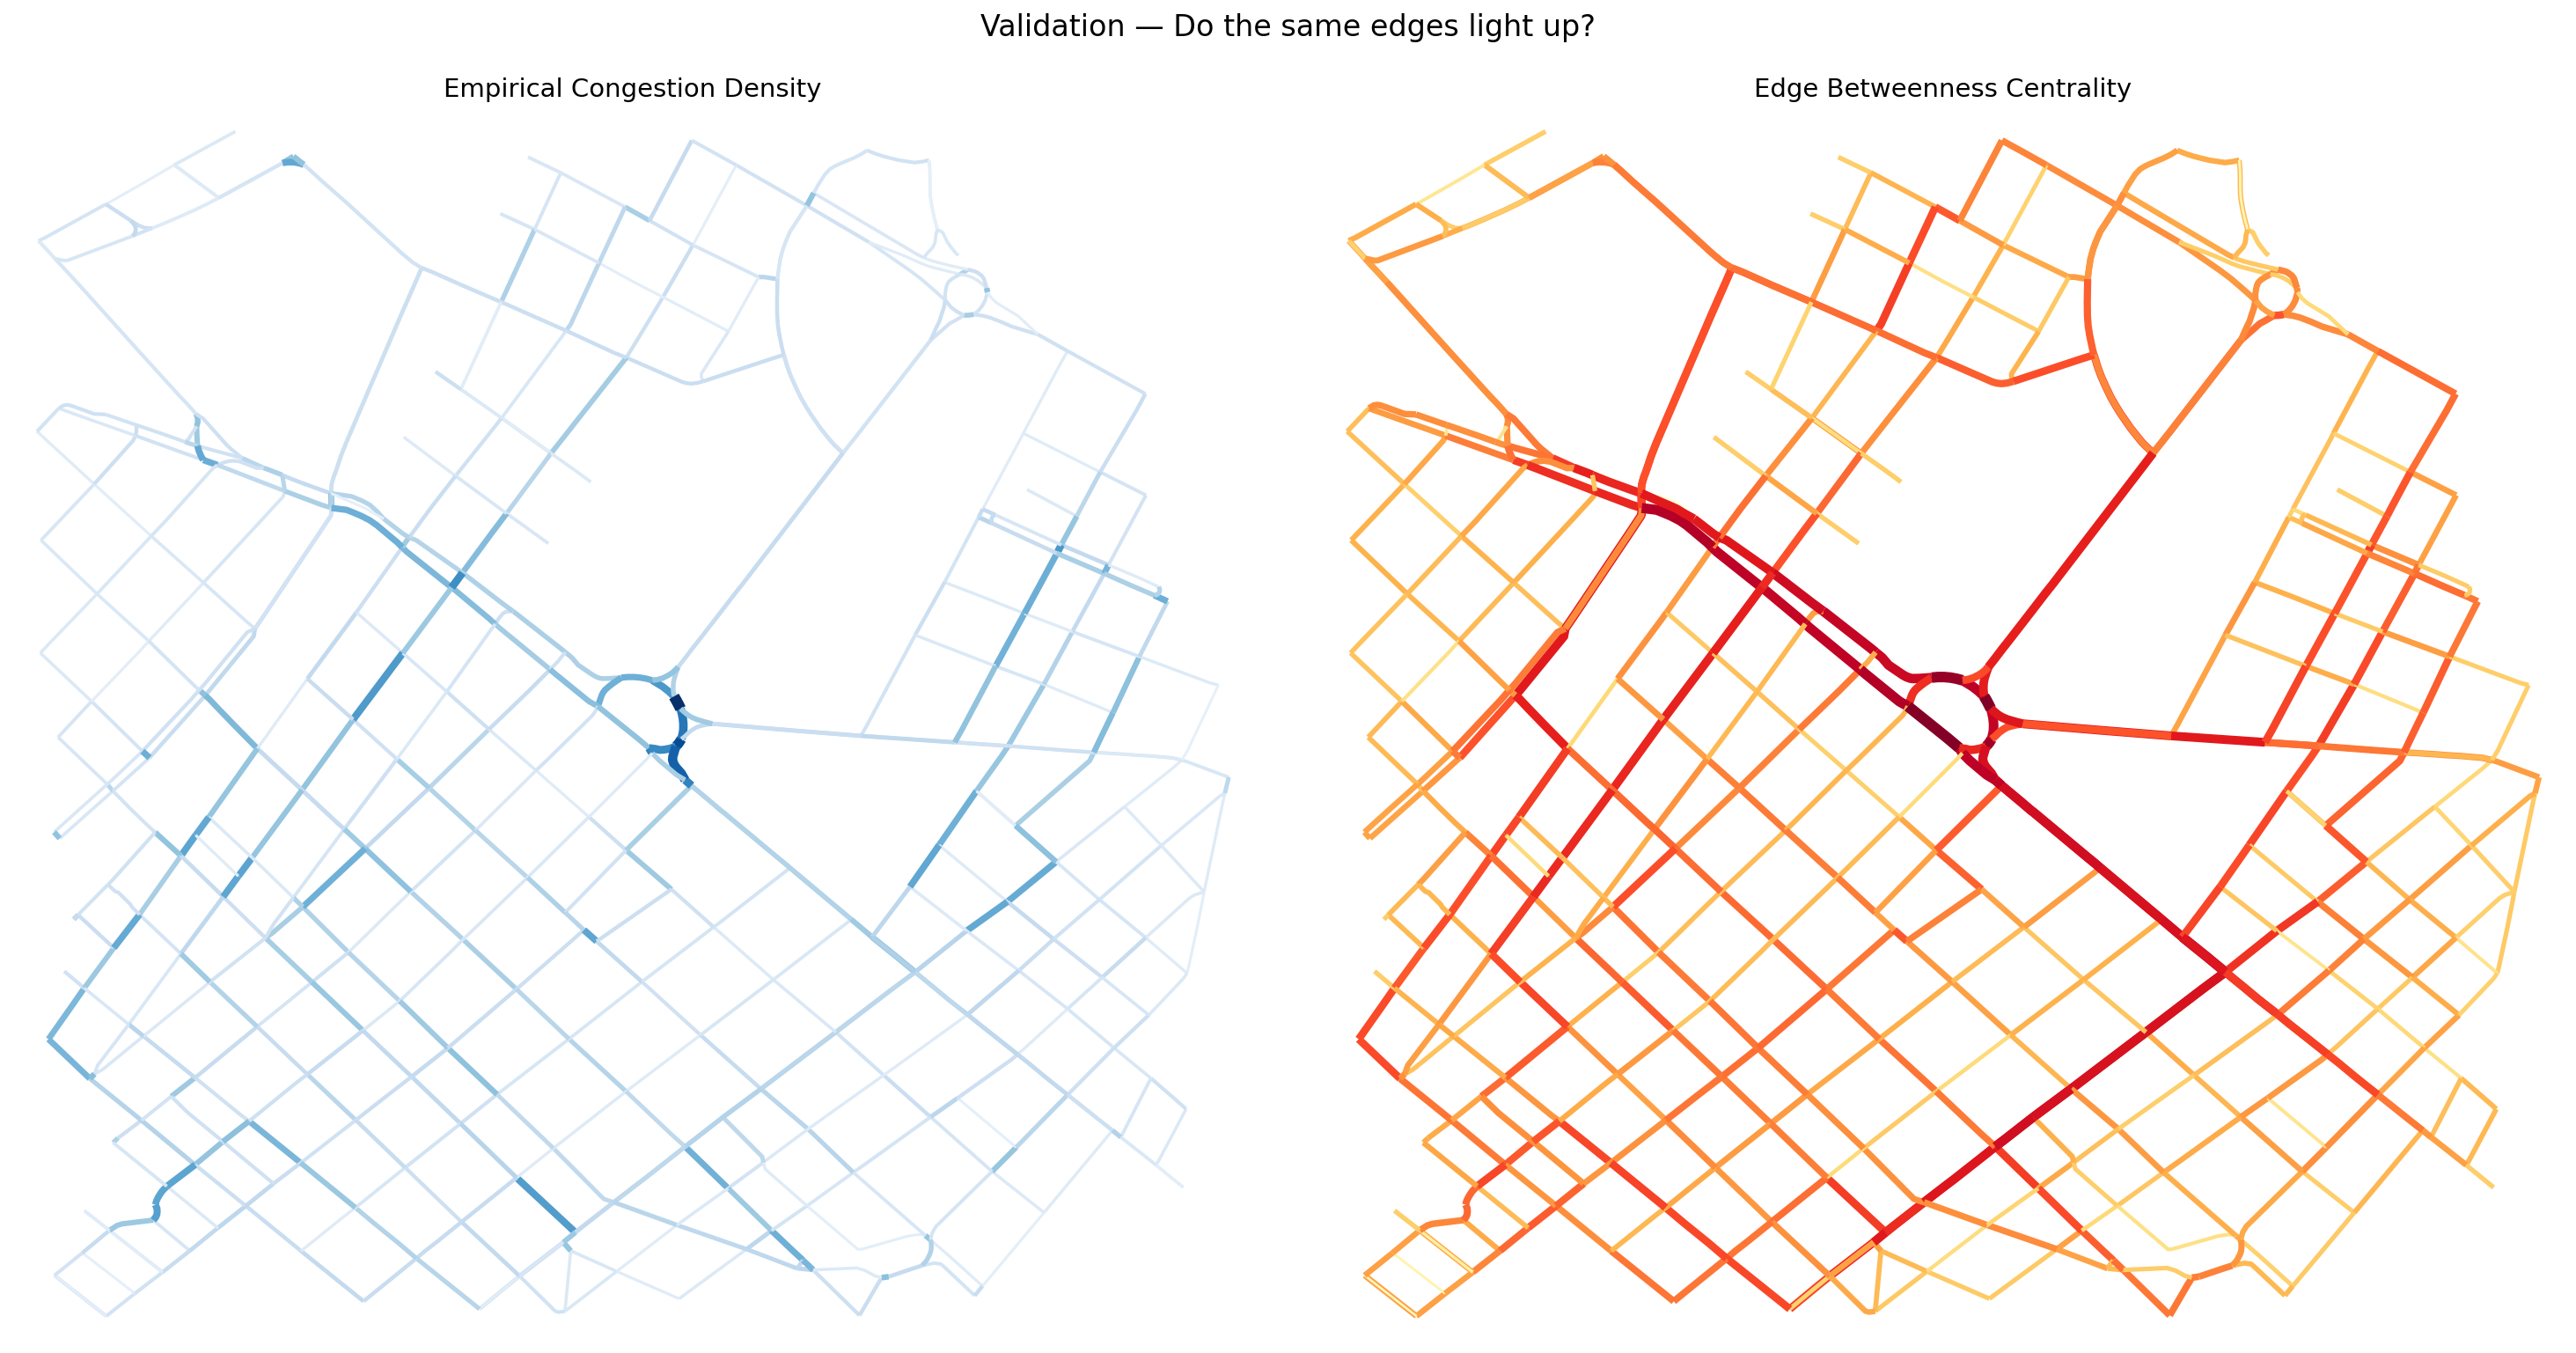
\includegraphics[width=\textwidth]{cell_36_0.png}
    \caption{Side-by-side spatial comparison on the Plaza Italia validation network. Left: empirical congestion density averaged across 50 runs (Blues scale). Right: edge betweenness centrality from network structure alone (YlOrRd scale). The general trend holds (high-betweenness edges tend to also show higher empirical density), though the match is noisier than on the Corrientes network, consistent with the lower Spearman $r = 0.81$.}
    \label{fig:sidebyside_palermo}
\end{figure}

\begin{figure}[H]
    \centering
    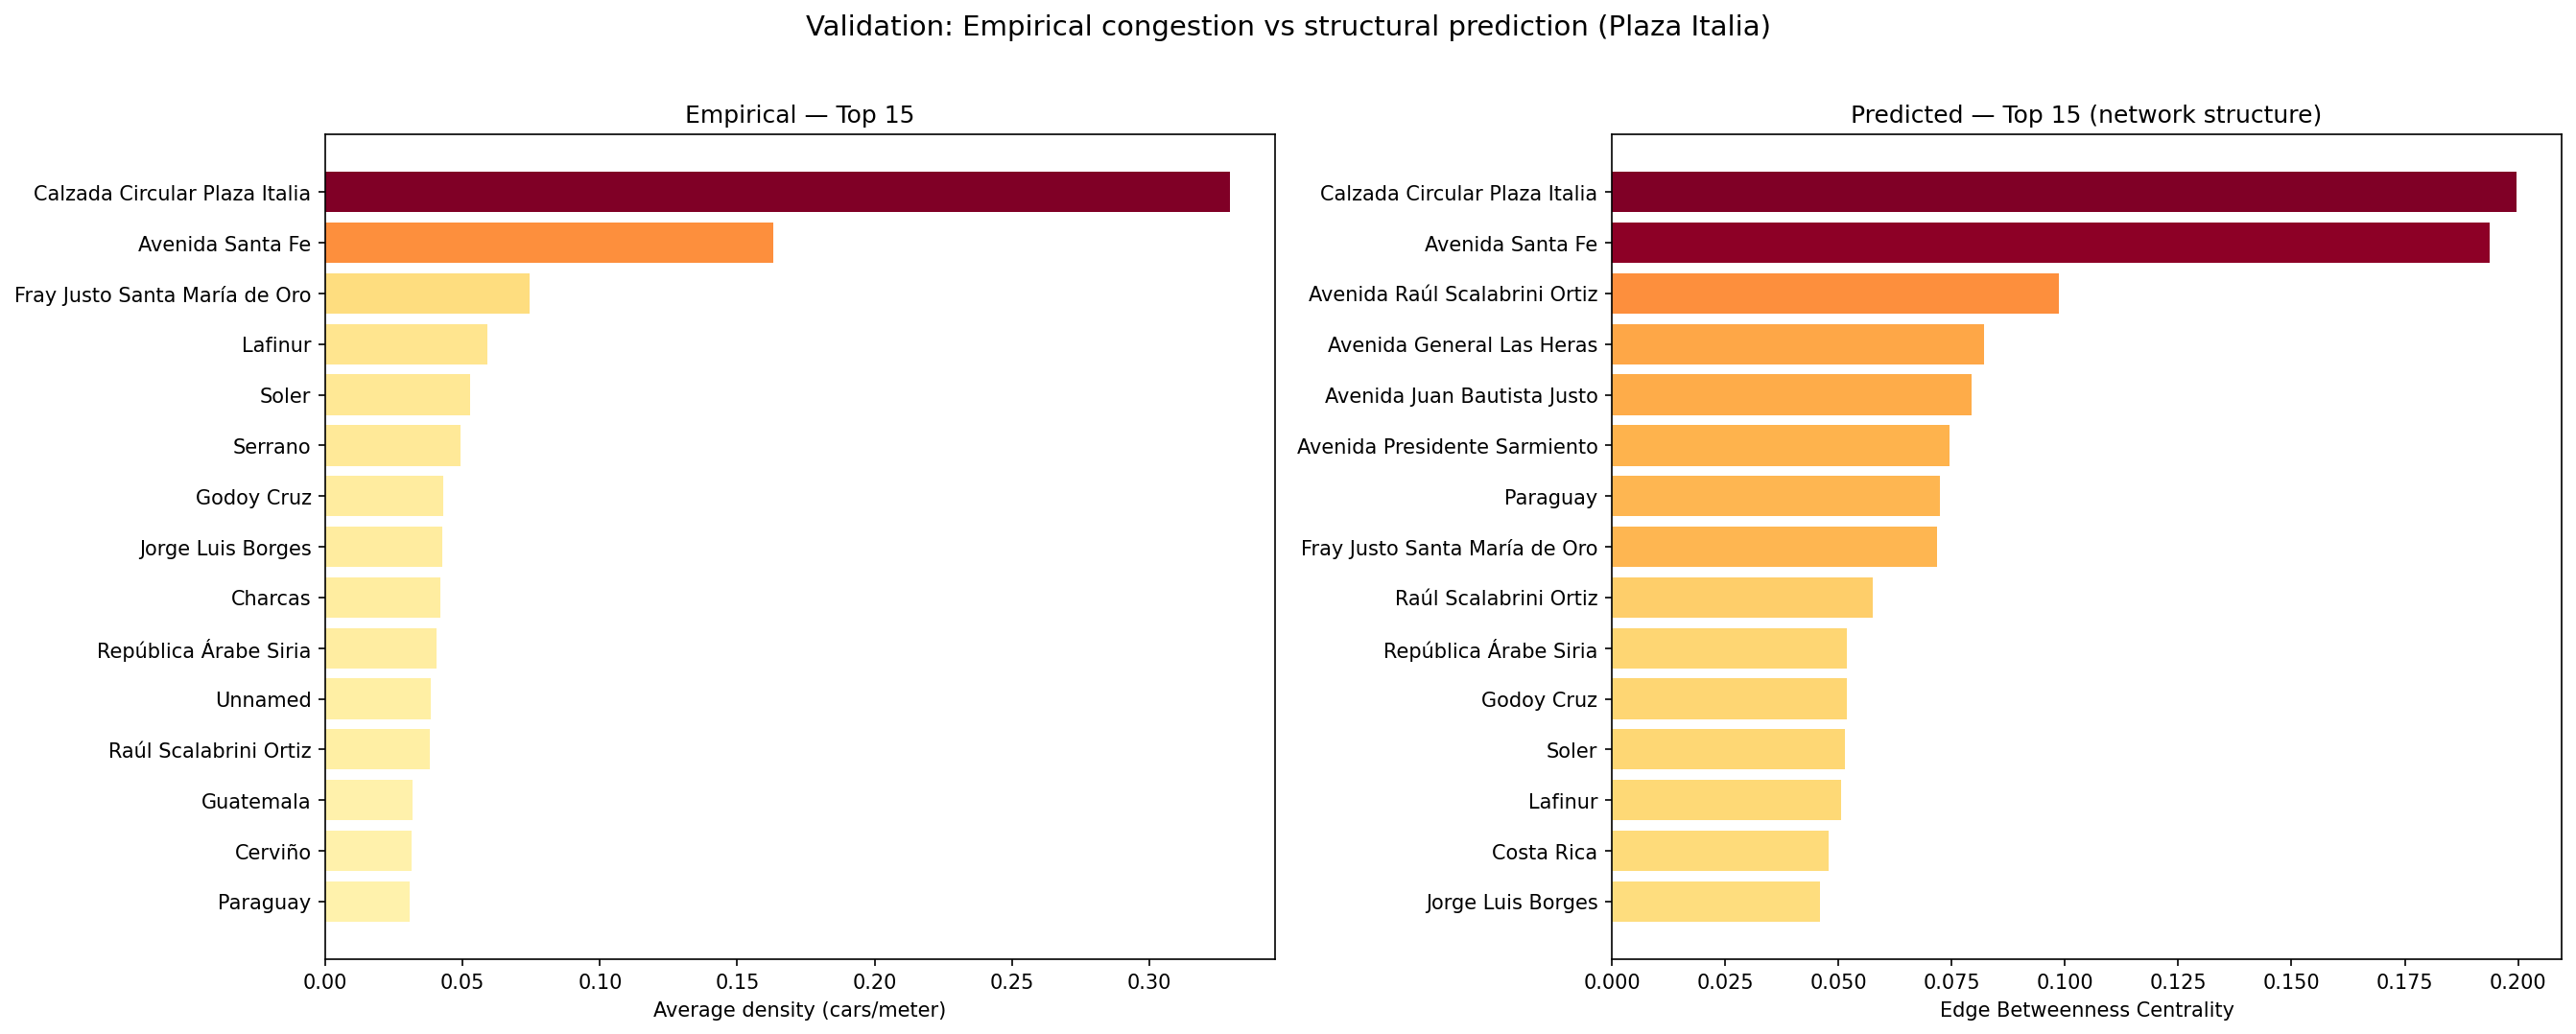
\includegraphics[width=\textwidth]{cell_37_0.png}
    \caption{Side-by-side comparison of the top 15 streets in the Plaza Italia validation network. Left: ranked by empirical congestion density (cars/meter) from 50 simulation runs. Right: ranked by edge betweenness centrality from network structure. Six streets appear in both lists (Calzada Circular Plaza Italia, Psje punto Santa Mar\'{i}a de Oro, Ra\'{u}l Scalabrini Ort\'{i}z, Rep\'{u}blica \'{A}rabe Siria, Jorge Luis Borges, and Latitud), confirming partial but meaningful overlap between empirical and structural rankings.}
    \label{fig:top15_palermo}
\end{figure}

\subsection{Discussion}

Edge betweenness centrality remains a strong predictor of empirical congestion density on the Plaza Italia network, with a Spearman correlation of $r = 0.81$ ($p < 10^{-139}$). This is slightly lower than the Corrientes result ($r = 0.88$), which is expected: the Palermo area has a less grid-like topology with more irregular intersections, so the relationship between shortest-path structure and congestion is noisier. Nevertheless, the correlation is still strong and highly significant.

The side-by-side bar chart (Figure~\ref{fig:top15_palermo}) shows substantial overlap between the streets ranked highest by empirical density and those ranked highest by edge betweenness. Streets that serve as connectors between major intersections appear in both lists, confirming that the structural prediction is not specific to the Corrientes network.

Since the prediction works on a network it was never calibrated on, the result is likely general: shortest-path routing concentrates traffic on high-betweenness edges regardless of the specific network layout. The slight decrease in correlation from Corrientes to Palermo suggests that network regularity (grid structure) strengthens the prediction, but even irregular networks exhibit the relationship clearly.


% ============================================================================
\section{Bonus: Gridlock Across Network Topologies}
\label{sec:gridlock}
% ============================================================================

\subsection{Motivation}

The previous sections showed that edge betweenness centrality predicts congestion on real road networks. But real road networks have a specific topology (roughly grid-like). A core question in network science is whether the same local update rule can produce different macro-level behavior depending on the structure of the system. Congestion on one road does not stay local; it propagates through the network as upstream edges back up and downstream edges starve. How far and how fast this propagation occurs depends on how the network is connected: a city built around a single central artery will experience network-wide gridlock more readily than one with many redundant paths. To test this, we apply the same Greenshields CA update rule to three synthetic network topologies and ask: how does congestion scale with the number of cars, and which topologies are most vulnerable to network-wide breakdown?

\subsection{Methodology}

We generate three synthetic graphs with approximately the same number of nodes (~140--150) but different connectivity structures. All edges have uniform properties (length = 100~m, speed limit = 30~km/h, lanes = 1) so that topology is the only variable. The three graphs are also constructed with similar node and edge counts (133--150 nodes, 504--592 directed edges) so that differences in the speed curves reflect topology, not network size. This is a deliberate simplification: real cities have varying road widths, speed limits, and network sizes, but uniform properties isolate the structural effect.

For each topology, we sweep the number of cars from 25 to 1000 in 11 steps. At each car count, we run 20 independent simulations of 100 steps each. After each step, we record the average speed fraction across all active cars: each car's speed divided by the free-flow speed on its current edge, so 1.0 means free flow and 0.0 means stopped. We report steady-state values: the average speed fraction computed over only the last 20\% of simulation steps, by which point the initial transient (cars spreading out from random starting positions) has settled and the network has reached a roughly stable congestion level. We also report the standard error of the mean across runs, which is appropriate because we are estimating the expected average at each car count, not the variability of individual runs.

\subsection{Graph Topologies}

\begin{figure}[H]
    \centering
    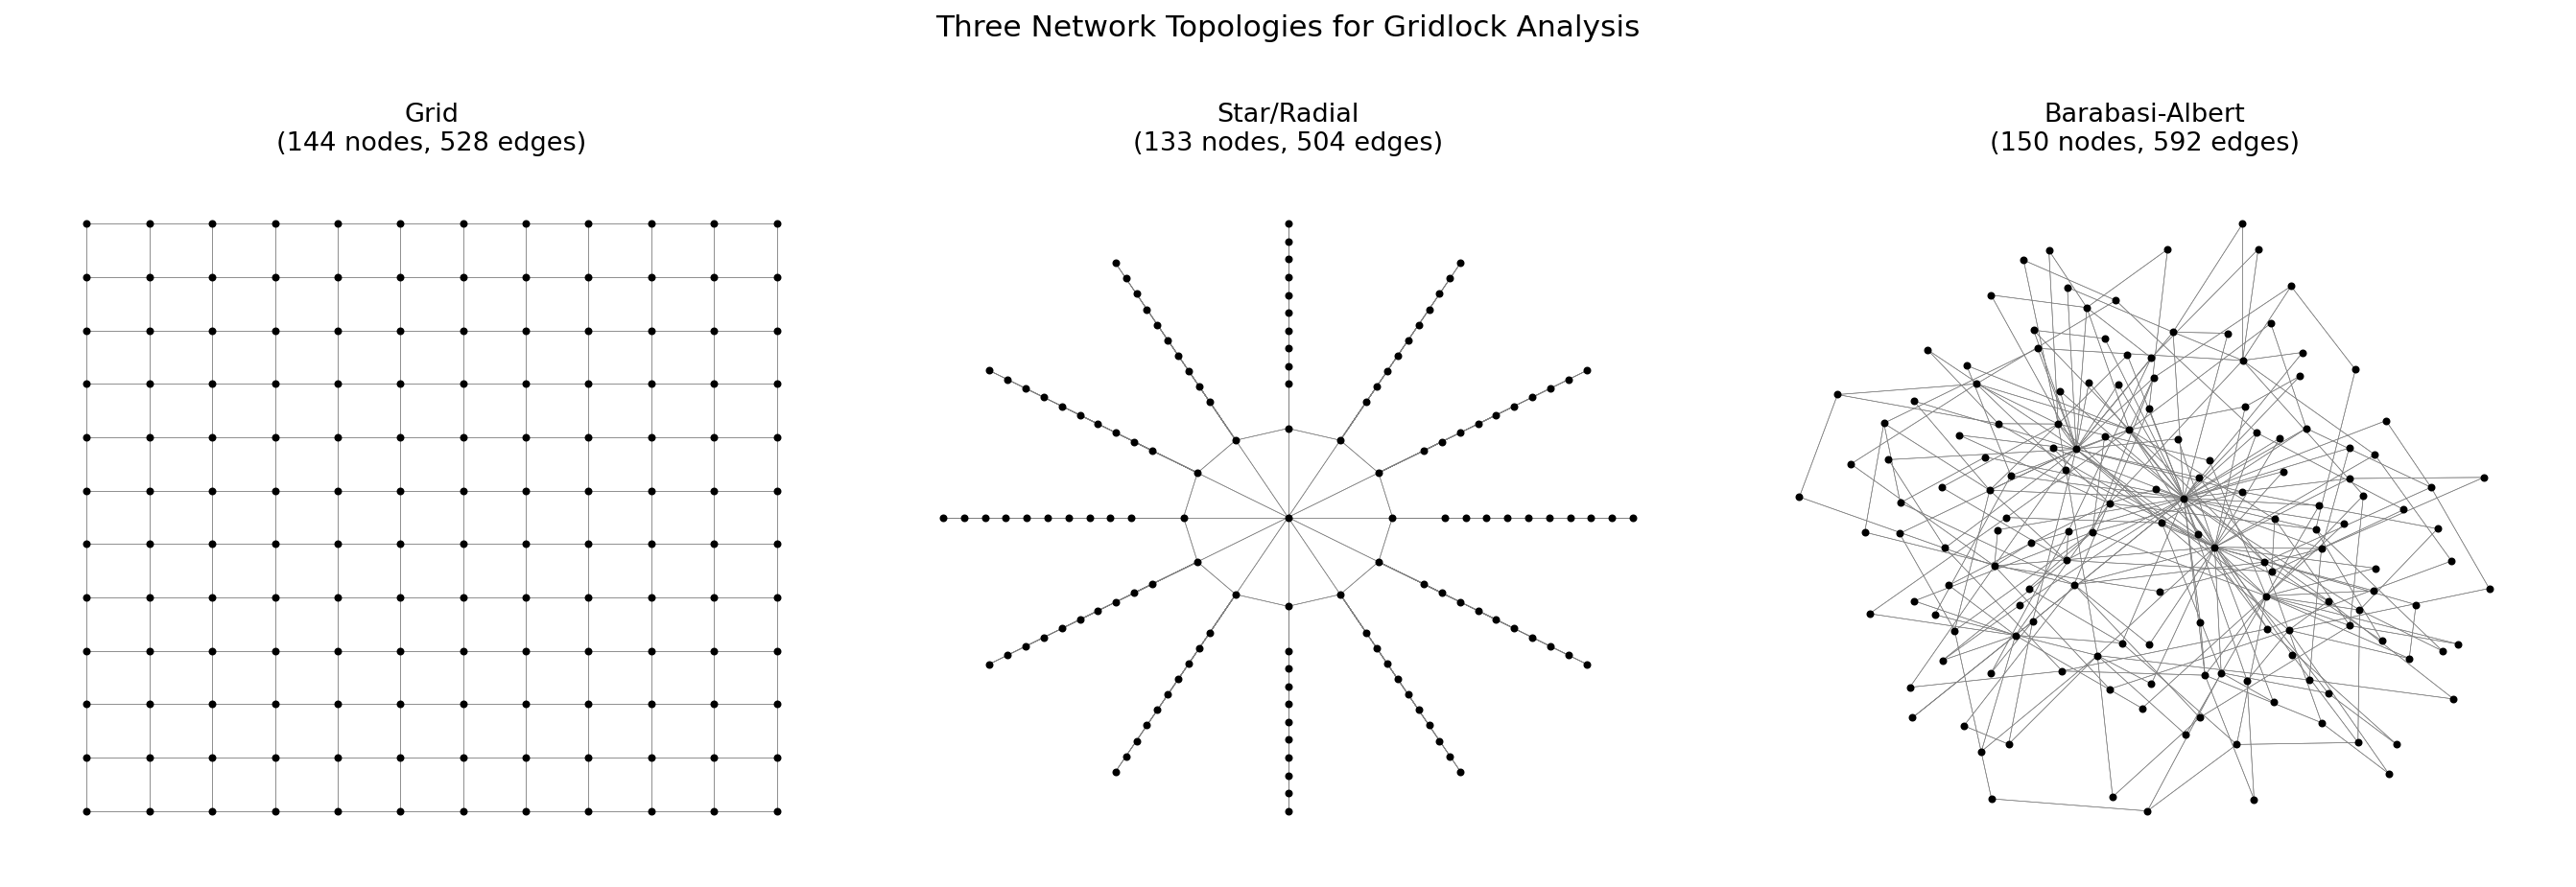
\includegraphics[width=\textwidth]{cell_40_1.png}
    \caption{The three synthetic network topologies used for gridlock analysis. Left: a 12$\times$12 grid representing a Manhattan-style city with high path redundancy. Center: a hub-and-spoke radial network where cross-sector traffic funnels through a central hub. Right: a Barab\'{a}si-Albert scale-free network where a few high-degree hubs attract disproportionate traffic. All edges have identical properties (100~m, 30~km/h, 1 lane) so topology is the only variable.}
    \label{fig:topologies}
\end{figure}

\begin{itemize}
    \item \textbf{Grid} (144 nodes, 528 directed edges): A $12 \times 12$ grid with bidirectional edges. Every node has degree 4 (or less at boundaries). Represents Manhattan-style cities with regular, uniform connectivity.
    \item \textbf{Star/Radial} (133 nodes, 504 directed edges): A central hub connected to 12 ring nodes, which form a circle and each have 10 leaf nodes in chains. Cross-sector traffic must pass through the hub. Represents European-style cities with radial road patterns.
    \item \textbf{Barab\'{a}si-Albert} (150 nodes, 592 directed edges): Generated by preferential attachment, producing a scale-free degree distribution. A few high-degree hub nodes have many connections, while most nodes have few. Represents cities with a few major arterial roads and many minor streets.
\end{itemize}

\subsection{Results}

\begin{figure}[H]
    \centering
    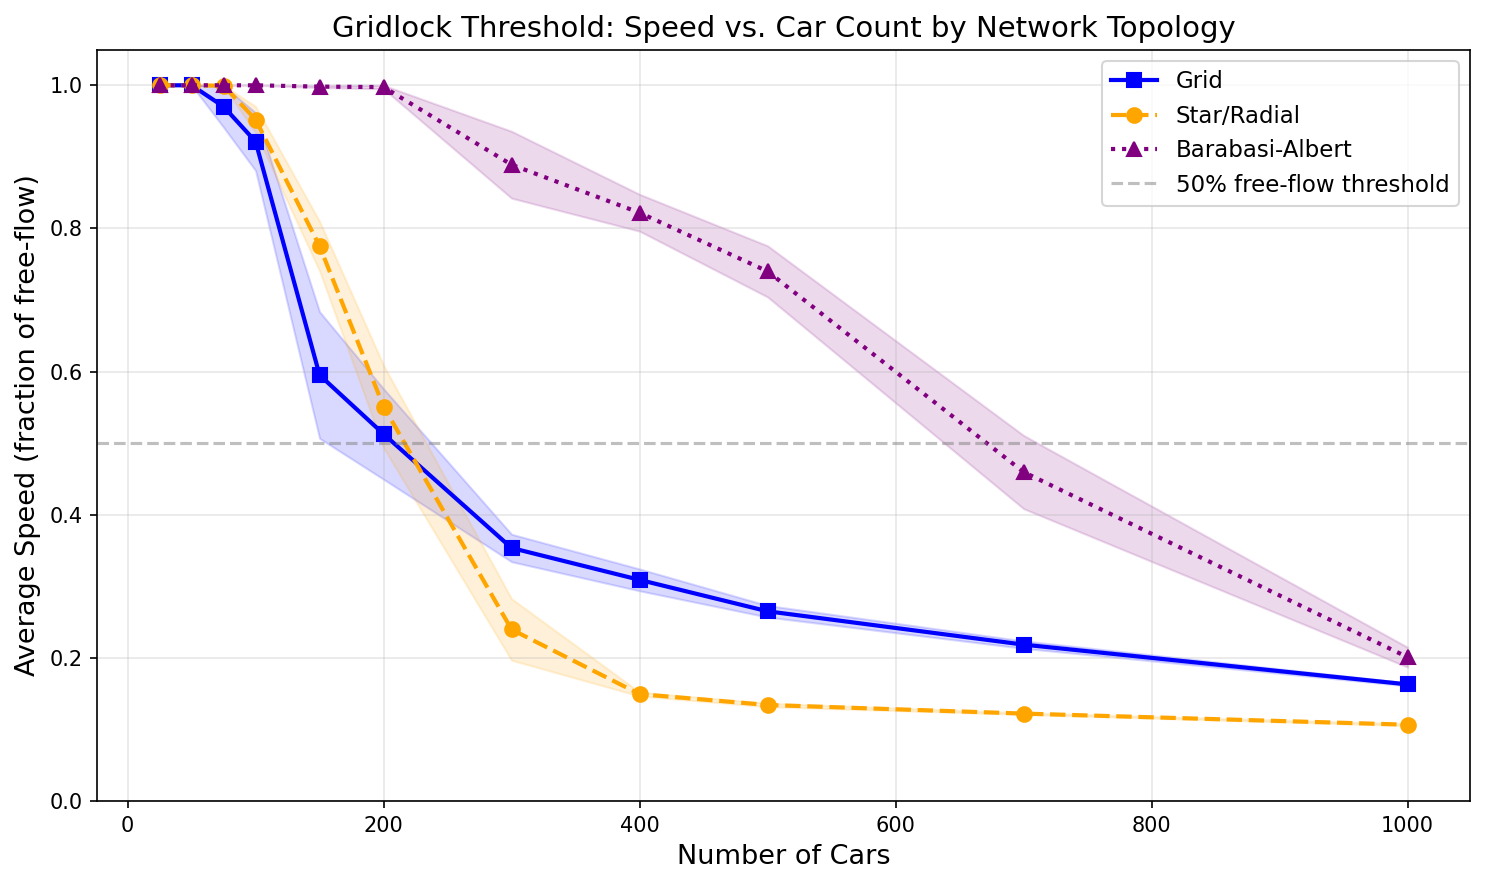
\includegraphics[width=0.85\textwidth]{cell_42_0.png}
    \caption{Average speed (as fraction of free-flow) vs.\ number of cars for each network topology. Shaded bands show $\pm 1$ standard error of the mean across 20 runs. All three topologies start near 1.0 at low car counts but diverge sharply as car count increases, each exhibiting a qualitatively different congestion profile.}
    \label{fig:speed_vs_cars}
\end{figure}

The three curves in Figure~\ref{fig:speed_vs_cars} show three distinct congestion profiles:

\textbf{Star/Radial (orange):} The sharpest collapse. Speed drops almost vertically between 50 and 300 cars, falling from near-free-flow to below 0.2. This is the signature of a single bottleneck: once the central hub saturates, nearly all cross-sector traffic stalls simultaneously. There is no graceful degradation; the network is either flowing or gridlocked.

\vspace{0.5em}
\textbf{Grid (blue):} A steep initial decline followed by a \textbf{plateau}. Speed falls to around 0.3--0.4 by 200 cars, but then stabilizes in that range until roughly 500 cars before continuing to decline. This plateau suggests partial gridlock: the central rows and columns (where shortest paths concentrate) are congested, but peripheral routes still flow. The grid is congested but not fully stopped, a qualitatively different regime from the star's all-or-nothing collapse.

\vspace{0.5em}
\textbf{Barab\'{a}si-Albert (purple):} The most gradual decline. Speed stays near 1.0 well past 200 cars and decreases steadily without a sharp cliff. The network degrades incrementally as progressively lower-degree hubs saturate one by one, rather than collapsing at a single critical point. Beyond approximately 700 cars, all three topologies converge to near-zero speeds.

The tight standard error of the mean bands confirm that these differences are reproducible across runs.

\vspace{0.5em}
\subsection{Discussion}

The speed curves reveal three qualitatively distinct congestion regimes, each a consequence of topology:

\begin{itemize}
    \item \textbf{Star/Radial: catastrophic collapse.} The hub is a single point of failure. Once it saturates, congestion is self-reinforcing (dense edges slow cars, which keeps them on the edge longer, which increases density further) and the entire network grinds to a halt. The speed curve shows a sharp boundary between the ``flowing'' and ``gridlocked'' regimes.
    \item \textbf{Grid: partial gridlock with a plateau.} Shortest-path routing concentrates traffic on central rows and columns, which congest at relatively low car counts. But the grid's many parallel paths allow peripheral routes to keep flowing, stabilizing average speed at a mediocre level. The grid's redundancy is only partially useful here because our simulation uses static routing; with dynamic rerouting, the grid's alternative paths would become more effective.
    \item \textbf{Barab\'{a}si-Albert: gradual degradation.} The scale-free degree distribution means a few hubs have many edges and can absorb heavy traffic before saturating. As car count increases, hubs congest one by one in order of decreasing degree, producing a smooth decline rather than a sharp cliff. The many edges connecting low-degree peripheral nodes rarely appear on shortest paths and stay uncongested until very high car counts.
\end{itemize}

\vspace{0.5em}
The same update rule on three different topologies produces three different congestion profiles: the grid plateaus, the star collapses, and the BA network slopes down gradually.

\vspace{0.5em}
The BA network's resilience suggests a design principle for real cities: a road network with a few high-capacity arterial roads (hubs) connected by many smaller streets degrades more gracefully under load than either a uniform grid or a centralized radial layout. The hub roads absorb disproportionate traffic, and when one hub saturates, traffic redistributes to others rather than cascading into system-wide gridlock. Los Angeles exemplifies this pattern: its freeway system functions as a set of high-degree hubs (the 405, 101, 10, and 110 freeways) connecting a sprawling network of surface streets. Despite its reputation for traffic, the system handles enormous volumes precisely because congestion on one freeway does not immediately paralyze the rest of the network. Drivers have alternative arterials, and the load distributes across multiple high-capacity corridors. A city built around a single central boulevard (the star topology) would collapse far more readily under the same total traffic volume.


% ============================================================================
\section{Conclusion}
% ============================================================================

The original ChatGPT-generated simulation's binary threshold fails to capture how real traffic behaves. By implementing the Greenshields speed-density model as a cellular automaton on a network graph, we obtain continuous congestion dynamics that can be meaningfully measured and visualized.

Edge betweenness centrality predicts empirical congestion density because cars follow shortest paths, and edges on many shortest paths carry more traffic. This relationship holds across both tested real-world network topologies (Spearman $r = 0.88$ on Corrientes, $r = 0.81$ on Palermo), suggesting it is a general property of shortest-path routing on road networks.

The gridlock analysis on synthetic networks demonstrates that network topology determines the qualitative character of congestion: the star/radial collapses catastrophically, the grid reaches a partially-congested plateau, and the scale-free BA network degrades gradually. The same Greenshields update rule produces three distinct congestion regimes depending on topology, showing that network topology, not the update rule, determines how congestion plays out.

% ============================================================================
\section*{AI Use Statement}
% ============================================================================
\addcontentsline{toc}{section}{AI Use Statement}

In this project, AI was only used to format and structure the code and written text. All analysis decisions, experiment design, and interpretation of results are my own.

\bibliography{references}

\end{document}
